\documentclass[a4paper, 12pt, oneside]{report}
\usepackage[T1]{fontenc}
\usepackage[utf8]{inputenc}
\usepackage{lmodern}
\usepackage{layout}
\usepackage{emptypage}
\usepackage{fancyhdr}
\usepackage[spanish,activeacute]{babel}
%\usepackage[Conny]{fncychap}
%\usepackage{graphicx}
\usepackage{subfigure} % subfiguras
\usepackage{caption}
\usepackage{mathtools}
\usepackage{hyperref}
\usepackage[a4paper,top=3cm, bottom=3cm, inner=2.5cm, outer=2.5cm]{geometry}
\usepackage{listings}
\usepackage[spanish]{babel}
\usepackage{url}
\usepackage{float}
\usepackage{multirow}
\usepackage{rotating} 
\usepackage{color}
\usepackage{colortbl}
\usepackage[table]{xcolor}
\usepackage[spanish]{babel}
\usepackage{enumerate}
\usepackage{enumitem}
\usepackage{multicol}
\usepackage{mwe}
\usepackage[acronym, nonumberlist]{glossaries}
\makeglossaries

\makeatletter
\renewcommand{\@makeschapterhead}[1]{%
%  \vspace*{50\p@}%
  \vspace*{0\p@}%
  {\parindent \z@ \raggedright
    \normalfont
    \interlinepenalty\@M
    \Huge \bfseries  #1\par \nobreak
%    \vskip 40\p@
    \vskip 15\p@
  }}
\makeatother

\renewcommand{\baselinestretch}{1.4}
\setlength{\headheight}{16pt} 
\captionsetup{justification=justified}
\pretolerance=1000

\chead[]{}
\rhead[]{}
\renewcommand{\headrulewidth}{0.5pt}

\pagestyle{empty}

\title{Pr\'acticas Docentes de Rob\'otica en el Entorno JdeRobot-Academy}
\author{Pablo Moreno Vera}

\lstset{
	float=hbp,
	basicstyle=\ttfamily\small,
	columns=flexible,
	tabsize=4,
	frame=single,
	extendedchars=true,
	showspaces=false,
	showstringspaces=false,
	numbers=none,
	numberstyle=\tiny,
	breaklines=false,
	breakautoindent=true,
	captionpos=b
}
\setcounter{tocdepth}{4}
\setcounter{secnumdepth}{4}

\definecolor{lightgray}{gray}{0.9}

\begin{document}
%%%%%%%%%%%%%%% Portada %%%%%%%%%%%%%%%%%%%%
\begin{titlepage}
	\begin{center}
		\vspace*{3mm}
		\begin{center}
			
\includegraphics[width=0.8\linewidth]{figures/logo.jpg}
		\end{center}
		\vspace{6.5mm}
		
		\fontsize{15.5}{14}\selectfont ESCUELA TÉCNICA SUPERIOR DE INGENIERÍA DE TELECOMUNICACIÓN
		\vspace{13mm}
		
		\fontsize{14}{14}\selectfont DOBLE GRADO EN INGENIERÍA DE SISTEMAS \\ DE TELECOMUNICACIÓN Y ADMINISTRACIÓN Y DIRECCIÓN DE EMPRESAS
		
		\vspace{55pt}
		
		\fontfamily{lmss}\fontsize{15.7}{14}\selectfont \textbf{TRABAJO FIN DE GRADO} 
		
		\vspace{15mm}
		\begin{huge}
			Nuevas Prácticas Docentes de Robótica en el \\ \vspace{0.4cm} Entorno JdeRobot-Academy
		\end{huge}
		
		\vspace{15mm}
		
		\begin{large}
			Autor: Pablo Moreno Vera
			
			Tutor: José María Cañas Plaza
			
			\vspace{10mm}
		\end{large}
		\begin{normalsize}
			Curso académico 2018/2019		
		\end{normalsize}
		\vspace{10mm}
		
	\end{center}
	
\end{titlepage}

\pagenumbering{Roman}

%%%%%%%%%%%%%%% Agradecimientos %%%%%%%%%%%%
\newgeometry{top=1.6cm,left=2cm,right=2cm}
\chapter*{Agradecimientos}
\setlength{\parskip}{1ex}

Me gustaría aprovechar esta parte del trabajo para dar a conocer un poquito de mí, de mi esencia y qué la ha causado. Para dar a conocer por qué he conseguido llegar hasta donde estoy y por haber conseguido llegar siendo quién soy.

Quiero dar las gracias, en primer lugar, a mis padres, quienes nunca han dudado de mí, ni por un segundo. Me han apoyado en todo momento y me han llevado de la mano hasta donde estoy. Me han demostrado que hay que pelear cada paso, porque nadie te va a regalar nada y menos si es algo que merece la pena. Han conseguido sacar una sonrisa de los momentos más dolorosos y demostrarme que, a veces, sólo es necesario sonreír. Me han enseñado la importancia de la familia y sé que sin ellos no lo habría logrado. Hemos pasado malos momentos, de todo tipo, y hemos salido de ello juntos. Juntos hemos derrotado a una enfermedad que se lleva millones de vidas en el mundo y que, en muchas ocasiones, no tiene cura como es el cáncer y, aun teniendo que estudiar junto a la camilla de mi padre en el hospital hemos conseguido derrotarlo y aprobar mis asignaturas. Este título lo hemos conseguido los 3 juntos, gracias por todo.

También quiero dar las gracias a mi tutor José María, por mostrarme el camino hacia el éxito. Por enseñarme que sin esfuerzo y estudio no se alcanza ningún objetivo propuesto y por mostrarme la robótica. La ciencia que me ha mostrado un lugar de interés perpetuo, un campo en continuo desarrollo y en el cual, tras un año en el desarrollo de este Trabajo de Fin de Grado, sólo tengo conocimiento de una infinitésima parte. Te agradezco aquellas palabras de interés por mí al terminar tu examen para que decidiera unirme ti para que mostrases la robótica. Has hecho de mí una persona trabajadora y constante durante todas las semanas de reuniones contigo.

Quiero agradecer a mi familia los momentos de tranquilidad y locura que me aportáis. Sólo con aparecer hacéis que desconecte de todo y me dé cuenta de que no estoy solo, que tengo gente que me quiere a mi alrededor y no es fácil de encontrar en personas que no eliges, sino que forman parte de ti al nacer. Aun así, estaré siempre agradecido por pertenecer a ese pequeño sitio del mundo en el que estáis vosotros.

Gracias a mi pareja, Vida, por enseñarme que la felicidad puede estar en unos ojos. Por hacerme sonreír con una mirada y hacer que olvide todo lo que me rodea. Sin el descanso que me das no habría aguantado la presión y no lo habría conseguido. Me has ayudado con asignaturas de las que ni siquiera comprendías lo que te contaba y, aun así, sin ti no habría llegado aquí. Eres mi lugar de descanso al que acudir cuando todo lo demás tiembla.

Me gustaría dar las gracias a todas las personas que habéis aportado un poquito en mi vida, que habéis conseguido hacer de mí una persona que está escribiendo un Trabajo de Fin de Grado para terminar una carrera de 4 años en la que muchos no confiaban pudiese finalizar. Muchas gracias a ti, Gabriel, por enseñarme que hay personas que te acompañan por el camino y no te abandonan. A todos vosotros, gracias.

La última mención es para las personas que me han guiado desde las estrellas todos los días de mi vida, que me dan su amor desde el cielo y que me han visto convertirme en quién soy. Gracias a mis abuelos que me cuidan a cada paso que doy y que, aunque no puedan decirme cómo se sienten al verme, me dan fuerzas para enfrentarme a cualquier dificultad que he encontrado y que me encontraré durante el camino que me queda por recorrer hasta verlos de nuevo. Y sobre todo a ti abuela que, aunque el Alzheimer haya apartado tu consciencia de mí y el azar se haya llevado tu vista, sé perfectamente que tu alma ya está con el abuelo y con ella puedes verme y darte cuenta lo mucho que os echo de menos.

Gracias a todos.
\restoregeometry


%%%%%%%%%%%%%%% Resumen %%%%%%%%%%%%%%%%%%%%
\chapter*{Resumen}
\setlength{\parskip}{1ex}

Debido al auge de la robótica en la actualidad, cada vez encontramos productos desarrollados mediante la robótica a nuestro alrededor. Por ello se acrecenta la necesidad de especialistas en este campo. Es por esto que surgen plataformas y entornos dedicados a llevar el campo de la robótica a estudiantes de distintas edades. En claro ejemplo es el JdeRobot-Academy, el cual pne a disposición de los alumnos universitarios y pre-universitarios un conjunto de ejercicios que representan un problema específico de la robótica, de una manera sencilla, completa y eficaz.

Este Trabajo de Fin de Grado se ha centrado en el desarrollo de una nueva práctica para el entorno de JdeRobot-Academy, así como una completa reestructuración y optimización de una de las prácticas ya presente en el entorno. Para cada práctica se ha desarrollado una solución de referencia.

Para la nueva práctica incluida, llamada \textit{Chrono}, ha sido necesario el completo desarrollo del nodo académico, así como su interfaz gráfica, la conexión de sensores y actuadores del robot con el nodo académico y la sincronización del simulador con las grabaciones procedentes de \textit{ROS-Kinetic} para la visualización del robot F1 a vencer.
Esta práctica permite al alumno enfrentarse al problema de captación y procesado de imágenes, además de preparar un algoritmo de control de movimiento del robot.

Para la optimización y mejora de la práctica llamada \textit{Follow Road}, fue necesario una reestructuración de su interfaz gráfica para introducir una visualización de la imagen procesada por el alumno y la integración de una pausa académica, así como el desarrollo de un algoritmo nuevo de conexión de sensores y actuadores para dar soporte a los \textit{drivers} proporcionados por \textit{ROS-Kinetic}.
Para esta práctica se ponen a disposición del alumnos todos los materiales para que pueda centrarse exclusivamente en los problemas de captación y procesado de imágenes y de la realización de un movimiento controlado por parte del dron para que siag de una manera eficiente la carretera.
\cleardoublepage

%%%%%%%%%%%%%%% Ìndices %%%%%%%%%%%%%%%%%%%%
%\cleardoublepage
%\renewcommand{\tablename}{Tabla}
%\renewcommand{\listtablename}{\'Indice de tablas}
%\tableofcontents

%\cleardoublepage % ͭndice de figuras
%\addcontentsline{toc}{chapter}{\listfigurename}
%\listoffigures

%\cleardoublepage % ͭndice de tablas
%\addcontentsline{toc}{chapter}{\'Indice de tablas}
%\listoftables 
\cleardoublepage
\tableofcontents % indice de contenidos
\listoffigures % indice de figuras
\addcontentsline{toc}{chapter}{\'Indice de figuras} % para que aparezca en el indice de contenidos

\cleardoublepage

%%%%%%%%%%%%%%% Acronimos %%%%%%%%%%%%%%%%%%%%
%\include{0-Acronimos}

%%%%%%%%%%%%%%% Cap��tulos %%%%%%%%%%%%%%%%%%
\pagestyle{fancy}
\pagenumbering{arabic}
\setlength{\parindent}{6mm}

\lhead[]{CAP\'ITULO \thechapter. INTRODUCCI\'ON}
\chapter{Introducción}\label{cap.introduccion}
El Trabajo Fin de Grado (TFG) descrito a continuación pertenece a un entorno educativo para la enseñanza de la programación de robots. En este capítulo se desarrollará el contexto en el que se sitúa este proyecto y la motivación que he llevado a su desarrollo. Es preciso comenzar con una explicación a grandes rasgos sobre qué es la robótica y sus aplicaciones en la sociedad.

La parte funcional más importante en la robótica viene suministrada por el software. Dentro del software podemos destacar diferentes elementos como los simuladores, las bibliotecas de código y los middlewares de robótica, los cuales serán descritos en la segunda sección del capítulo. En la tercera sección de este capítulo se describirá la situación actual de la robótica en el panorama educativo y en el entorno de JdeRobot-Academy, en el cual está desarrollado este TFG. La intención principal de su desarrollo es extender este entorno docente con nuevos ejercicios que representen un problema en la robótica. En cuanto al desarrollo de un sistema robótico, hay numerosas cuestiones a las que enfrentarse y solucionar. A la mayoría de estos problemas se enfrenta y soluciona el entorno docente y se oculta al estudiante, para que se pueda centrar en los algoritmos que dotarán vida al robot.

\section{Robótica}
A lo largo de la historia, la ciencia y la tecnología han sido utilizadas por el hombre para facilitarle la vida. Para ello, ha ideado, desarrollado y construido herramientas y máquinas empleándolas para reducir su carga de trabajo. En este entorno se desarrolla la robótica, que es la rama de la tecnología basada en la utilización de la informática para el diseño y desarrollo de sistemas automáticos que faciliten la vida al ser humano e, incluso, llegar a sustituirle en algunas tareas determinadas. La robótica incluye conceptos de disciplinas diversas, como la física, las matemáticas, la electrónica, la mecánica, la inteligencia artificial, la ingeniería de control, etc. Gracias a todas estas disciplinas involucradas unidas convenientemente se pueden diseñas máquinas que ejecuten comportamientos autónomos según el propósito para el que han sido desarrolladas. Estas máquinas autónomas se denominan "Robots".

El término "Robot" fue concebido por Isaac Asimov en 1950. Desde entonces estos sistemas autónomos han experimentado un crecimiento exponencial en cuanto a complejidad, versatilidad, autonomía y, sobre todo, en su incorporación a una gran diversidad de ámbitos. Los sistemas operados por el ser humano comienzan a incorporar un sistema de control específico programable que permiten el desarrollo de tareas repetitivas o con un gran riesgo para las personas, englobando tareas básicas y de difícil realización, hasta la actualidad, en la cual existe un gran marco de ejemplos en los que se integran la robótica y multitud de campos y tareas. Los robots comerciales e industriales realizan las tareas de una manera más exacta o más barata que las personas. También son utilizados en trabajos peligrosos, sucios tediosos para el ser humano. Gracias a esto, se trata de un campo en crecimiento constante.

\begin{figure}[H]
	\begin{center}
		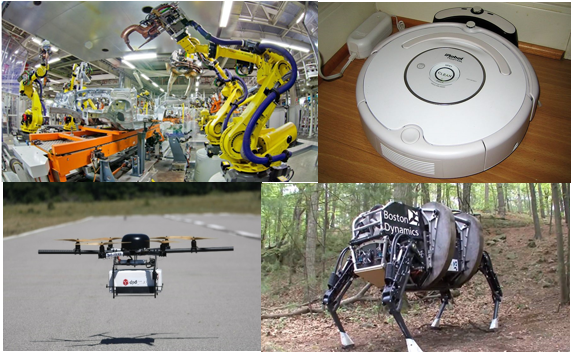
\includegraphics[width=0.8\textwidth]{figures/robots.png}
		\caption{Robots modernos}
		\label{fig.robots}
	\end{center}
\end{figure}

Ya se ha comentado la importancia de los robots en la actualidad en el aspecto industrial, pero tal el crecimiento que está experimentando la robótica que está comenzando a cobrar una gran importancia en aspectos menos especializados como el entorno doméstico. Cabe destacar el desarrollo de robots para facilitar la vida al ser humano, un ejemplo está ilustrado en la Figura 1.1. Las aspiradoras robóticas (Roomba, Dyson, Xiami, ...) han tenido un éxito rotundo en la realización de una actividad doméstica necesaria para la vida del ser humano. Otro éxito de la robótica en la actualidad es el desarrollo de coches autónomos. Este hecho se ha conseguido paulatinamente mediante la incorporación de tecnología cada vez más sofisticada a los automóviles. En este aspecto cabe destacar los módulos de aparcamiento automático, el park assist o los asistentes de conducción autónoma (autopiloto Tesla), o los prototipos de coches autónomos (Apple o Google). Otro ámbito en el que la robótica ha sido introducida es el militar, donde se han incorporado robots de rescate o para la desactivación de bombas. En la medicina se ha desarrollado el robot DaVinci, que permite operar desde cualquier parte del mundo con una precisión mayor a la humana. En el ámbito de la logística Amazon ha desarrollado una flota de robots de almacén que consiguen trasladar los pedidos a lo largo de sus almacenes. Tal es el punto de crecimiento de la robótica que se están desarrollando robots con "comportamientos inteligentes" como el robot Asimo de Honda (Figura 1.2) que pueden interactuar con humanos, ya sea como asistente para el hombre o con fines experimentales como la locomoción bípeda.

\begin{figure}[h]
	\centering
	\begin{minipage}[h]{.48\linewidth}
		\centering
		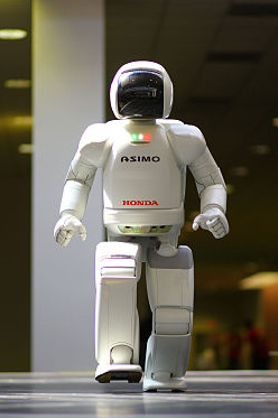
\includegraphics[width=.5\linewidth, height=7cm]{figures/asimo.png}
		\captionof{figure}{Robot Ásimo}
		\label{fig:asimo}
	\end{minipage}
	\begin{minipage}[h]{.48\linewidth}
		\centering
		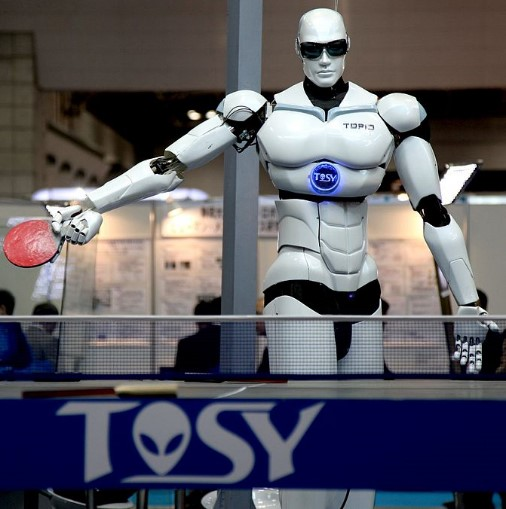
\includegraphics[width=.7\linewidth, height=7cm]{figures/topio.jpg}
		\captionof{figure}{Robot TOPIO}
		\label{fig:topio}
	\end{minipage}
\end{figure}

Los ámbitos en los que se puede aplicar la robótica es tan extenso como la imaginación de las personas dedicas a su creación, gracias a esto ámbitos en los que sólo podríamos imaginar automatizadas ahora son operadas totalmente con robots con resultados superiores a los de cualquier humano, como la agricultura de precisión mediante drones con análisis de imágenes térmicas y multiespectral para aumentar el rendimiento de las explotaciones agrícolas o el control de los productos industriales mediante el procesado de imágenes de la producción o la automatización de aplicaciones anestésicas de bajo nivel e, incluso, competiciones deportivas de robots.

Debido al gran potencial que tiene esta rama de la ciencia cobra una gran importancia la necesidad de dominarla. Gracias a ella ganaremos en comodidad, economía e, incluso, saludo. Es importante advertir de la importancia de la robótica en el futuro, ya que será la llave que abrirá la puerta a la humanidad hacia un mundo más seguro y sencillo mediante la automatización.

\section{Software Robótico}
Para que los robots puedan ser controlados de una manera eficaz el comportamiento del software que los controla debe ser robusto. Para ello se divide en distintas capas (\textit{drivers}, \textit{middleware} y aplicaciones), cuya arquitectura será distinta según su aplicación final.

Debido al gran desarrollo de la robótica, los robots actuales ya no precisan del control del ser humano para su funcionamiento, en la actualidad tienen comportamientos autónomos que les permiten realizar las tareas sin la mediación de terceros. Esto es posible gracias al minucioso desarrollo del software que compone los sistemas complejos del robot, algo parecido a una inteligencia autónoma. El desarrollo del software robótico parte de ciertas tareas o requisitos como son los circuitos de retroalimentación, control, búsqueda de caminos, localización o filtrado de datos entre otras muchas.

En los últimos años se han creado una gran cantidad de plataformas de desarrollo de software para las aplicaciones robóticas, también llamados /textit{middleware} robóticos. Los simuladores son otra parte importante para el desarrollo de software robótico ya que permiten realizar pruebas y depurar los fallos para programar una versión funcional del robot antes de ser fabricado. Esto supone un gran ahorro en costes. Estos componentes son vitales para generar el conjunto de comandos que componen la funcionalidad del robot, por ello entraremos en detalle en el siguiente apartado. Por último, las bibliotecas son necesarias para guardar los comandos que componen el funcionamiento del robot.

\subsection{Middlewares robóticos}
Los \textit{middleware} robóticos pueden definirse como entornos o \textit{frameworks} para el desarrollo de software pare robots. Se trata de software que conecta aplicaciones o componentes software para soportar aplicaciones complejas y distribuidas. Para controlar los sensores y actuadores de los robots estos entornos incluyen \textit{drivers}, arquitectura software para las aplicaciones que se van a crear, bloques de funcionalidad robótica ya resuelta, además de simuladores, visualizadores... Por ello al \textit{middleware} se le suele conocer como "pegamento para software". Una de las tareas del \textit{middleware} es conectar el hardware, ya sea real o simulado, con la aplicación desarrollada. El \textit{middleware} más extendido en el mundo es ROS.

	\textbf{Robot Operating System (ROS)\footnote{\url{http://www.ros.org/}}}

Se trata de una plataforma de software libre para el desarrollo software de robots que proporciona la funcionalidad de un sistema operativo en un clúster heterogéneo como el control de dispositivos de bajo nivel, mecanismos de intercambio de mensajes entre procesos y la abstracción del hardware, necesarios para el desarrollo de la robótica. Aunque el \textit{framework} ROS se desarrolló para los sistemas UNIX, se ha adaptado para ser soportado en otros sistemas operativos como Fedora, Debian, Windows, Mac OS X, Arch, Slackware, Gento u OpenSUSE, llegando a permitir las aplicaciones multiplataforma. Gracias a esto el \textit{framework} ROS se ha convertido en el más utilizado.

Existen otros \textit{framework} interesantes como:

	\textbf{Orocos}\footnote{\url{http://www.orocos.org/}}

Permitiendo el control avanzado de máquinas y robots en C++.

	\textbf{Orca}\footnote{\url{http://orca-robotics.sourceforge.net//}}

Está orientado a componentes por lo que permite el desarrollo de aplicaciones más complejas. Se tratta de un proyecto de software libre.

	\textbf{Urbi}\footnote{\url{https://github.com/urbiforge/urbi}}

Es un \textit{middleware} multiplataforma de código abierto en C++ que permite desarrollar aplicaciones en sistemas completos y complejos. Trabaja de forma conjunta con ROS.

	\textbf{JdeRobot}\footnote{\url{https://jderobot.org/}}

Plataforma de desarrollo de apicaciones robóticas y de visión artificial que incluye nodos programados con varios lenguajes de programación (Python o C++) compatible con \textit{middleware} de comunicaciones como ICE o ROS.

\subsection{Simuladores robóticos}
Debido al gran coste que supone la fabricación del hardware del robot es preciso depurar los posibles errores que contenga el código, así como el funcionamiento del hardware antes de su fabricación. Por ello debe probarse el código en un simulador orientado al tipo de aplicación que estemos desarrollando. Gracias a los simuladores es posible probar este código sin tener que fabricar previamente el hardware. De esta manera cualquier mal funcionamiento del código del robot puede ser solventado evitando la rotura del hardware. Algunos de los simuladores más utilizados son:

	\textbf{Gazebo}\footnote{\url{http://gazebosim.org/}}

Se trata del simulador 3D de código abierto más extendido. Funciona bajo la licencia Apache 2.0 y tienen gran importancia su motor de renderizado avanzado, sus motores de física y su soporte para \textit{plugins} de robot y sensores, además de su amplio catálogo de robots con sus sensores y actuadores. Otro hecho importante es su soporte para ROS lo que permite probar el código real del robot n el simulador.

	\textbf{Stage}\footnote{\url{http://wiki.ros.org/stage}}

Es un simulador en dos dimensiones, integrable con ROS, que permite simular numerosos robots simultáneamente.

	\textbf{Webots}\footnote{\url{https://www.cyberbotics.com/}}

Simulador de róbotica avanzada en el que se pueden desarrollar modelos propios y su física, escribir sus conroladores y hacer simulaciones a gran velocidad. Un ejemplo es su soporte para el humanoide Nao.

\subsection{Diseñadores Gráficos}
A la hora de introducir los modelos de los robots desarrollados en el simulador, así como un mundo simulado para comprobar la adaptación del mismo al medio, es necesario el uso de software de diseño gráfico. Este software permite la creación del modelo del robot e introducirla en el simulador. Gracias a esto se pueden ahorrar una gran cantidad de costes a la hora de desarrollar robots debido a que cualquier fallo estructural puede ser solventado antes incluso de la fabricación del prototipo. Algunos de los diseñadores gráficos más utilizados son:

	\textbf{SketchUp}\footnote{\url{https://www.sketchup.com/}}

Se trata de un programa de diseño gráfico y modelado en tres dimensiones basado en caras. Su principal característica es la realización de diseños en 3D de manera sencilla. Además incluye una extensa galería llamada 3D Warehouse que incluye esquemas de objetos, texturas e imágenes descargables. Este sofware de diseño es multiplataforma y de pago.

	\textbf{Blender}\footnote{\url{https://www.blender.org/}}

Es una programa de diseño gráfico dedicado especialmente al modelado, iluminación, renderizado, animación y creación de gráficos tridimensionales. También dispone de composición digital utilizand la técnica procesal de nodos, edición de vídeo, escultura (incluyendo topología dinámica) y pintura digital. También puede utilizarse para desarrollo de videojuegos dado que consta de una motor de juegos interno. Inicialmente fue distribuido de manera gratuita pero sin el código fuente, con un manual de uso, aunque posteriormente pasó a ser de software libre. Blender es multiplataforma con soporte para GNU/Linux, Windows, Mac OS X, Android, Solaris, FreeBSD e IRIX.

\subsection{Bibliotecas}
En el desarrollo de software deben abordarse un gran abanico de problemas clásicas, básicas y específicas para cada aplicación. Esta tarea es muy tediosa si hay que abordarla desde cero y requeriría un gran tiempo enfrentarse a ellas. Para evitar la repetición de problemas a la hora de desarrollar una aplicación, existen bibliotecas de código. Estas bibliotecas ofrecen conjuntos de implementaciones de código que permiten solucionar de manera directa ciertos problemas contenidos en su código. Esto permite al programador ahorrar una gran cantidad de tiempo para solucionar problemas que ya han sido solucionados anteriormente. Las bibliotecas pueden vincularse a un programa o a otra biblioteca en distintos puntos del desarrollo (bibliotecas estáticas) o durante la ejecución del programa (bibliotecas dinámicas). Algunas bibliotecas utilizadas en robótica son:

	\textbf{OpenCV}\footnote{\url{http://opencv.org/}}

Se trata de una biblioteca de código abierto que aborda problemas de visión artificial. Originalmente fue desarrollada por Intel y escrita en C++. En la actualidad contiene de interfaces en C++, Python, Java y MATLAB, además dispone de más de quinientas funciones que abarcan áreas de la visión artificial como reconocimiento de objetos y facial, calibración de cámaras y visión robótica y estéreo. Open CV es multiplataforma  y existen versiones para GNU/Linux, Mac OS X, Windows y Android.

	\textbf{OpenCV}\footnote{\url{http://pointclouds.org/}}

Es una librería utilizada para el procesamiento digital de imágenes RGBD mediante el tratamiento de nubes de puntos 3D. Entre sus numerosos algoritmos de última generación, se tratan problemas como filtrado, reconstrucción de superficies, ajuste de modelos, segmentación y estimación de características. Para simplificar el desarrollo, PCL se divide en bibliotecas de código  más pequeñas que pueden ser compiladas por separado. También es multiplataforma con soporte para Linux, Mac OS X, Windows y Android.

\section{Docencia en robótica}
La robótica con fines educativos está adquiriendo una gran importancia en la actualidad en la enseñanza preuniversitaria. Esto es debido a que su aprendizaje está disponible para estudiantes de cualquier nivel, el único requisito para estudiar robótico es la motivación por el desarrollo de aplicaciones. La robótica en el campo de la docencia cobra una gran importancia al ser una ciencia multidisciplinar, ya que incluye campos multidisciplinares como electrónica, informática, mecánica, física, ... Gracias a ello el estudiante adquiere una gran variedad de conocimiento de todas estas áreas. Además, proporciona una nueva visión del universo que le rodea, aprendiendo a distinguir los problemas y tomar una decisión al respecto.
En docencia primaria y secundaria se intenta despertar el interés del estudiante por la robótica, con la transformación de asignaturas teóricas tradicionales en asignaturas más prácticas e interactivas, ya que la robótica permite la recreación de problemas que les rodean y a través de los cuales pueden utilizar su creatividad y plasmar los conceptos teóricos que han adquirido.
En los centros de enseñanza primaria y secundaria se imparte robótica mediante plataformas físicas como los robots LEGO (Mindstorms, RCX, NXT, Evo, WeDo), placas Arduino, los kits de SolidWorks, etc.

\subsection{Docencias en la universidad}
En la docencia universitaria se imparte la robótica en distinto Grados y Postgrados en las escuelas de ingeniería. En España, se puede cursar la docencia robótica en el "Grado en Ingeniería Robótica" de la Universidad de Alicante, en los Grados de "Electrónica industrial y automática" o "Ingeniería Electrónica, Robótica y Mecatrónica" en distintas universidades, además de grados que están en desarrollo como el "Grado en Ingeniería Robótica Software" que imparte la Universidad Rey Juan Carlos desde el mes de Septiembre. Sin embargo, la docencia en robótica se reserva, mayoritariamente, para los Postgrados, dado que se trata una ciencia muy especializada. Existen varios Másteres destacados en cuanto a la docencia de robótica como el "Máster de Visión Artificial", el "Máster Universitario en Ingeniería Mecatrónica", o el "Máster Universitario en Automática y Robótica".
Dentro del ámbito internacional pueden encontrarse distintas universidades orientadas a robótica como el MIT, Carnegie Mellon University, Standford o Geordia Institute of Technology. También existen asociaciones prestigiosas como ACM (Association for Computing and Machinery) y la IEEE-CS (IEEE Computer Society) que ven la robótica como una ciencia imprescindible en estudios de ingeniería, informática y sistemas inteligentes.
En cuanto a la propia Universidad Rey Juan Carlos, cuenta con la plataforma docente JdeRobot, que consta de un entorno académico para la docencia de robótica llamado JdeRobot-Academy. Este entorno educativo se ha utilizado con éxito en distintas asignaturas como "Visión en Robótica" del Máster de Visión Artificial o en la asignatura Robótica del Grado de Ingeniería Telemática. Del mismo modo se han impartido talleres de aprendizaje para todos los públicos docentes, desde profesores de secundaria y primaria hasta estudiantes de secundaria pasando por trabajadores de distintas empresas. También se han impartido cursos de programación de drones para estudiantes universitarios.

\subsection{Entorno docente JdeRobot-Academy}
Los \textit{middleware} robóticos empleado para el desarrollo de este TFG son ROS y JdeRobot, que incluye el entorno académico JdeRobot-Academy\footnote{\url{https://jderobot.org/JdeRobot-Academy}}. Con este trabajo se ha pretendido extender sus posibilidades de aprendizaje, ampliándolo con dos nuevos ejercicios.
Los ejes en los que se apoya JdeRobot-Academy son:
\begin{enumerate}[label=\alph*)]
	\item Lenguaje Python (por su sencillez y potencia),
	\item simulador Gazebo (con distintos modelos de robot, tales como drones, formula1, brazos, aspiradoras, etc.), y
	\item foco en el algoritmo en vez de en el middleware, ocultando al estudiante los detalles de la infraestructura.
\end{enumerate}

El entorno JdeRobot-Academy cuenta con elenco de prácticas que abordan distintos problemas clásicos de la robótica. Para cada práctica se dispone de un componente académico que resuelve tareas auxiliares como la conexión con sensores y actuadores necesarios, la temporización o la interfaz gráfica y aloja el código del algoritmo del estudiante. De esta manera el estudiante se puede centrar en la solución del ejercicio exclusivamente. Cada nodo académico está formado por una parte específica oculta y el algoritmo con la lógica del robot del estudiante que se rellena en un fichero plantilla.

Debido a esta estructura, pueden distinguirse distintas capas en la composición de la práctica. La capa de nivel más bajo se le facilita al estudiante que sólo se centra en la capa superior donde se aloja la lógica del robot. Aunque esta capa más baja le viene dada al estudiante, es necesaria su implementación para poder dar solución a la práctica. En este aspecto se incluyen las conexiones de los sensores actuadores del robot, la interfaz gráfica, la temporización, el desarrollo del modelo del robot y un escenario que lo contenga, los plugins del modelo, los \textit{drivers} del mismo y la comunicación entre el simulador y el componente académico de alto nivel. Todo esto puede apreciarse en la Figura 1.4:

\begin{figure}[H]
  \begin{center}
    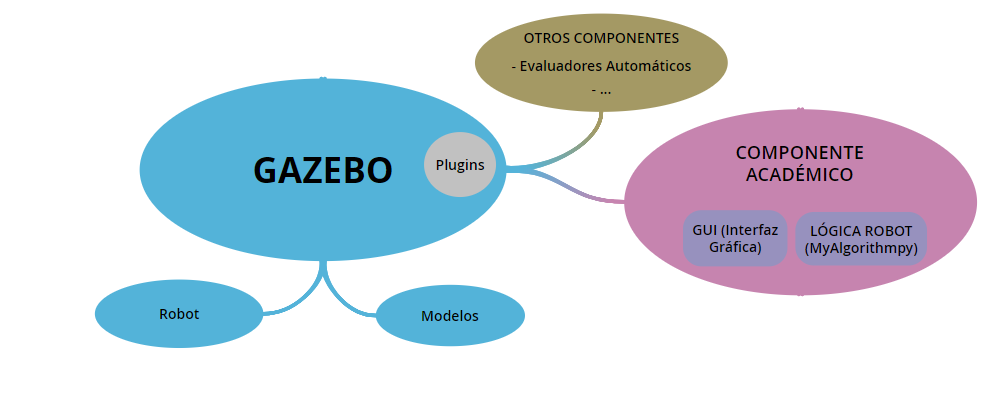
\includegraphics[width=0.9\linewidth]{figures/estructura_jde.png}
		\caption{Estructura de una práctica en JdeRobot-Academy}
		\label{fig.estructura}
		\end{center}
\end{figure}

Como se ha descrito anteriormente, en la Figura 1.4 se puede apreciar que la arquitectura software de las prácticas académicas facilita el desarrollo de las mismas por parte de los alumnos de manera que sólo se concentran en el desarrollo del algoritmo con la lógica del robot. El componente académico es el encargado de cargar en el simulador el código desarrollado por el alumno desde el fichero \textit{MyAlgorithm.py} y visualizar trazas que ayuden a la depuración del código como las imágenes procesadas, datos del láser o imágenes de la cámara integrada, dependiendo de la práctica.

El entorno usual para la realización de las prácticas es el simulador Gazebo, aunque las prácticas se han desarrollado de manera que puedan ser soportadas por robots reales sin realizar ninguna modificación, con los correspondientes drivers del robot. Gracias a esto, el código puede ser probado en robots reales. El sistema operativo base sobre el que se han desarrollado las prácticas es Linux dado que presenta una interfaz más sencilla a la hora de programar, por ello Linux cuenta con toda la infraestructura de las prácticas. 
Aunque en la actualidad se está terminando el entorno JdeRobot-Academy-Web en el que las prácticas docentes están almacenadas en un servidor y se puede acceder a ellas mediante el navegador. De esta manera se convierte al entorno JdeRobot en multiplataforma dotándolo de mayor accesibilidad. Esto es gracias al desarrollo de la interfaz web de Gazebo para la simulación, a la plataforma Jupyter (ver 3.6) que, mediante sus cuadernillos, han permitido trasladar las prácticas de JdeRobot-Academy al entorno docente JdeRobot-Academy-Web y al empleo de Dockers para dotar el entorno de un soporte multiplataforma.

Algunas de las prácticas que componen la plataforma son los siguientes:

\hspace{0.4\linewidth}
\textit{Follow Line}

\begin{figure}[H]
  \begin{center}
    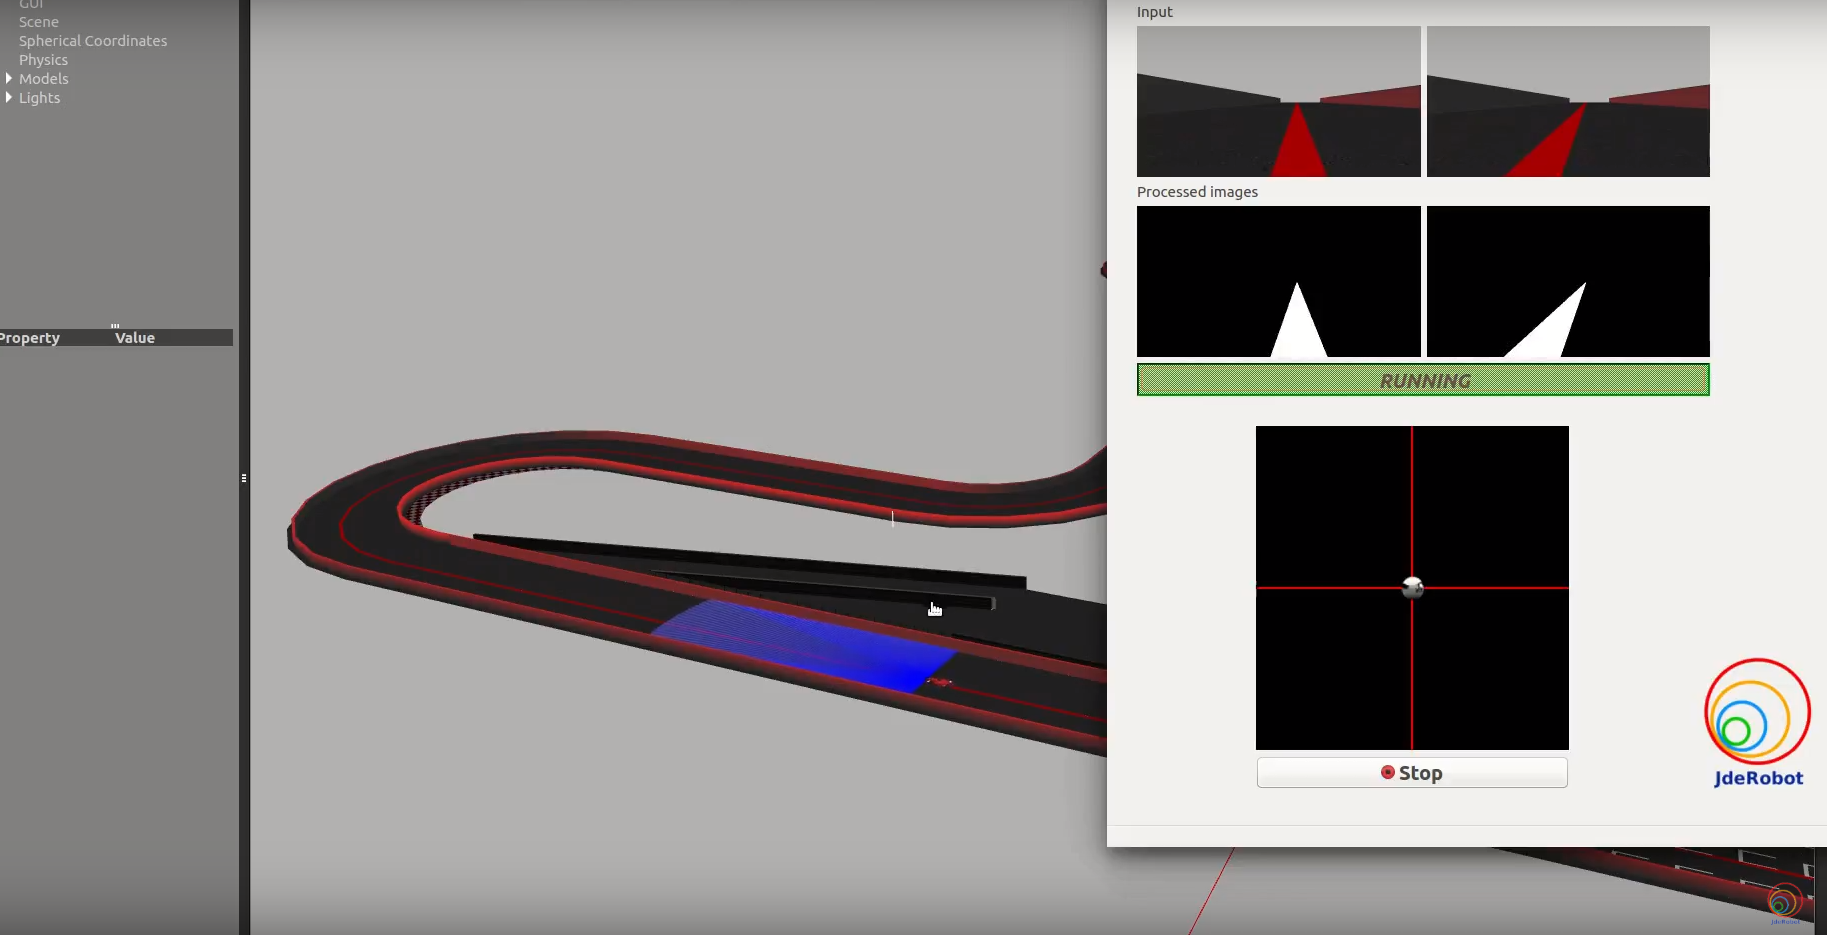
\includegraphics[width=0.95\textwidth]{figures/followline.png}
		\caption{Follow Line}
		\label{fig.followline}
		\end{center}
\end{figure}

Este ejercicio \textit{Follow Line} (Figura 1.5) trata de un robot coche Fórmula1 que consta de una cámara en su parte frontal por la que recoge imágenes. En su código se deben recoger las imágenes y procesarlas de manera que filtre la línea roja del circuito y la siga hasta que complete el circuito por completo \footnote{\url{https://youtu.be/QGO9oaoBVoA}}.

\vspace{4cm}
\hspace{0.40\linewidth}
\textit{Vacuum Cleaner}

\begin{figure}[H]
  \begin{center}
    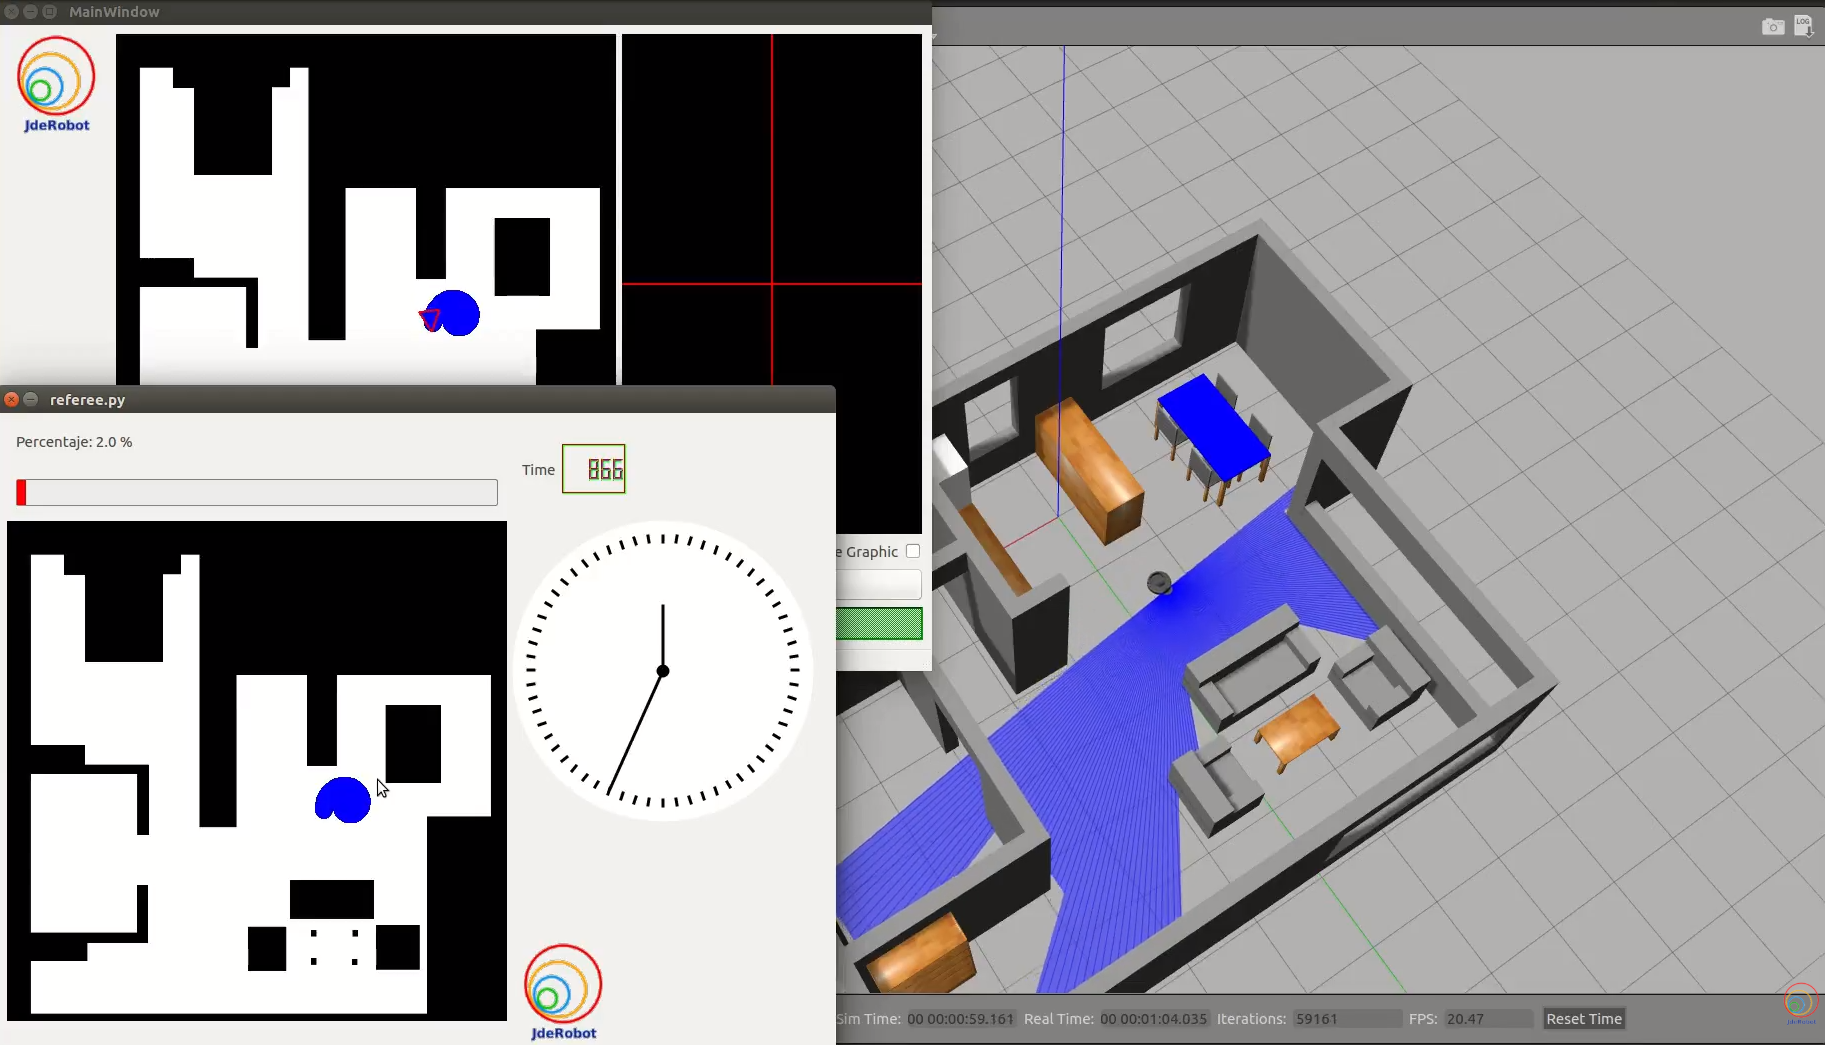
\includegraphics[width=0.50\linewidth, height=5cm]{figures/vacuumcleaner.png}
		\caption{Vacuum Cleaner}
		\label{fig.vacuumcleaner}
		\end{center}
\end{figure}

En este ejercicio \textit{Vacuum Cleaner} (Figura 1.6), el alumno debe recoger los datos del láser incluido en el modelo del robot aspiradora Roomba para que pase por el mayor área posible del escenario evitando la colisión con los obstáculos contenidos \footnote{\url{https://youtu.be/12muuY9JXLk}}.

\vspace{4cm}
\hspace{0.40\linewidth}
\textit{Visual Lander}

\begin{figure}[H]
  \begin{center}
    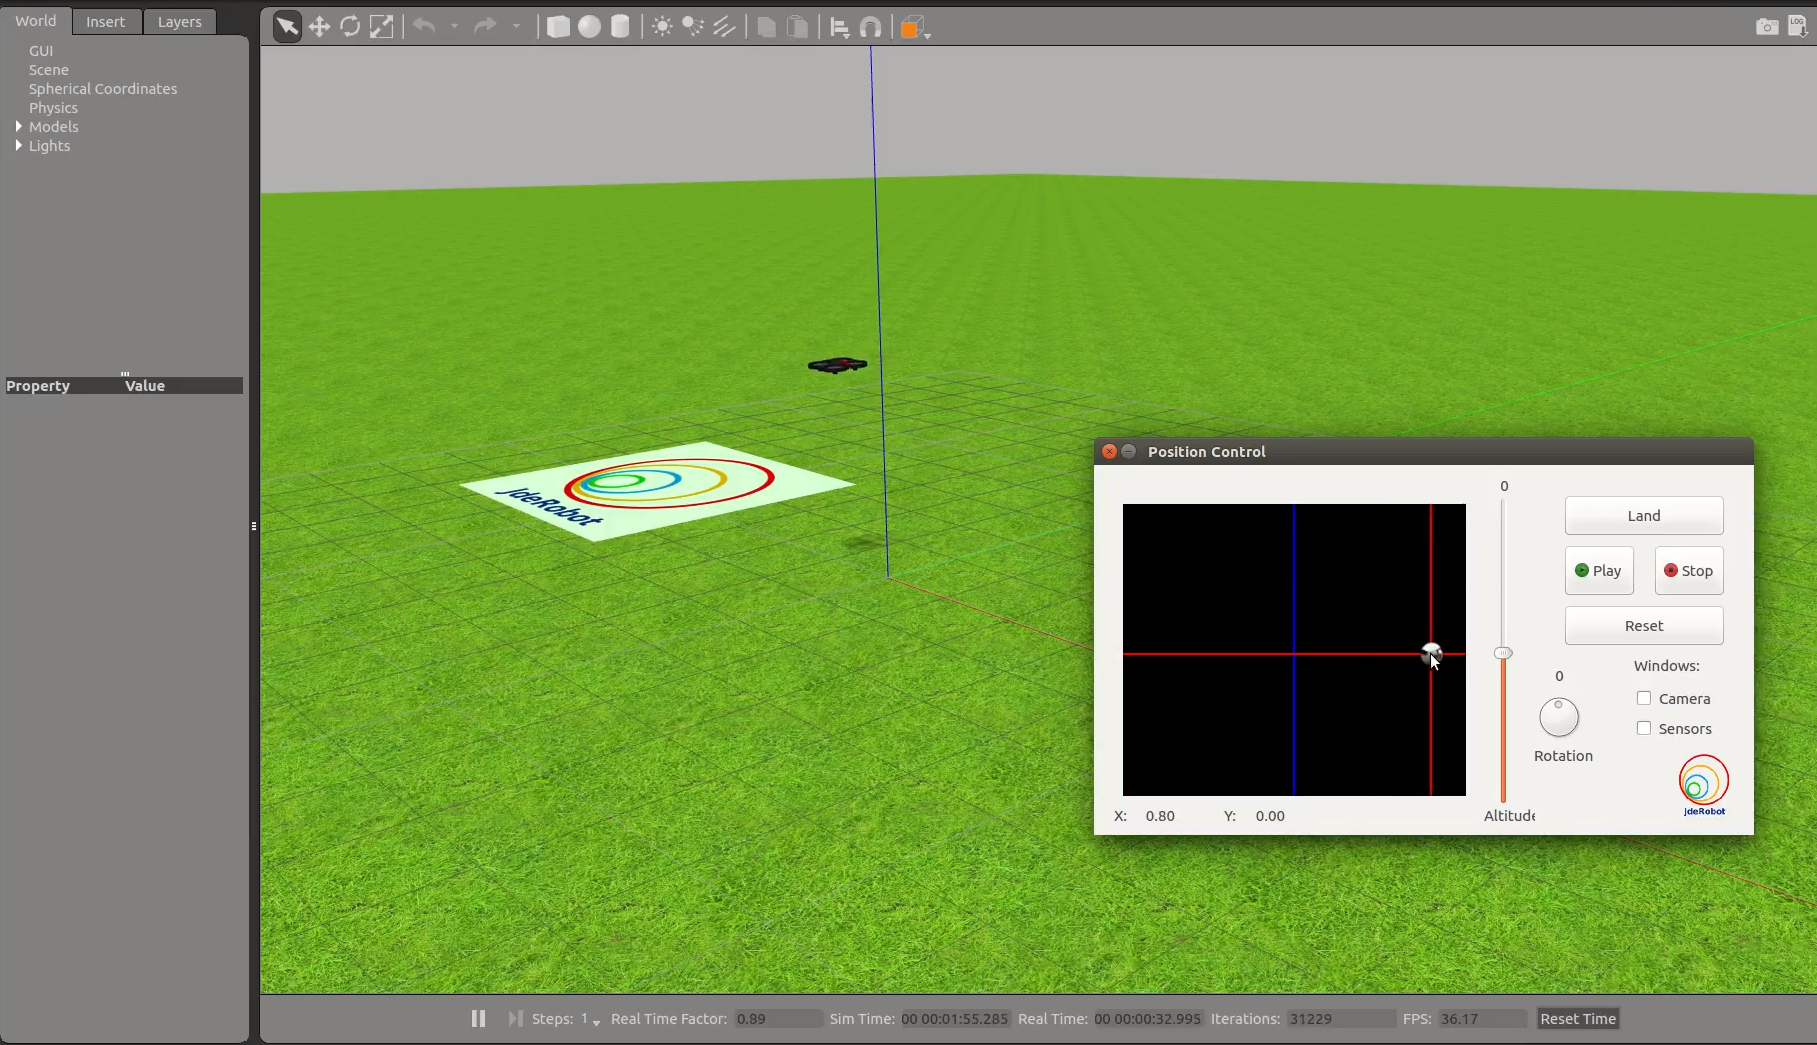
\includegraphics[width=0.50\linewidth, height=5cm]{figures/visuallander.png}
		\caption{Visual Lander}
		\label{fig.visual lander}
		\end{center}
\end{figure}

En este ejercicio \textit{Visual Lander} (Figura 1.7), el alumno deberá programar la lógica de un dron para que filtre las imágenes captadas por su cámara ventral y filtrarlas para distinguir una baliza y aterrizar controladamente sobre ella \footnote{\url{https://youtu.be/36pwaFYmDD0}}.

\vspace{4cm}
\hspace{0.40\linewidth}
\textit{Follow Turtlebot}

\begin{figure}[H]
  \begin{center}
    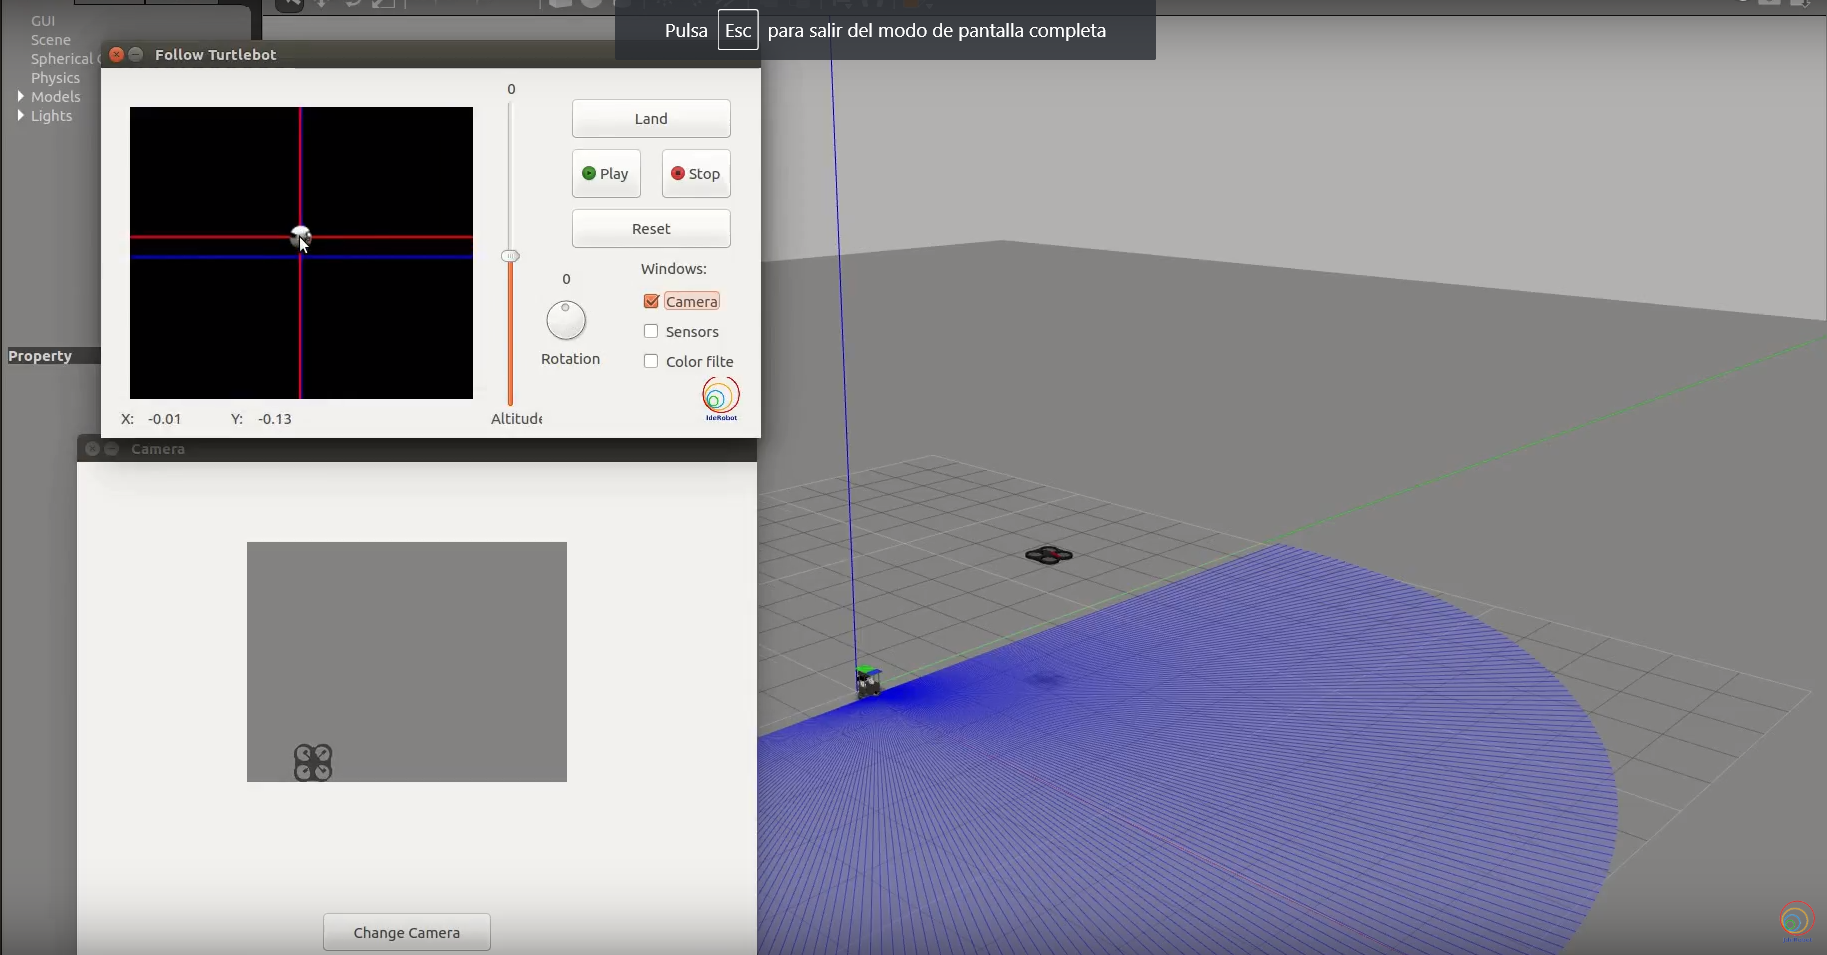
\includegraphics[width=0.50\linewidth, height=5cm]{figures/followturtlebot.png}
		\caption{Follow Turtlebot}
		\label{fig.followturtlebot}
		\end{center}
\end{figure}

Este ejercicio \textit{Follow Turtlebot} (Figura 1.8), consta de un escenario con un robot turtlebot teleoperado por el alumno y un dron. El código del algoritmo deberá dotar la inteligencia necesaria al dron para recoger las imágenes captadas por la cámara ventral del dron y filtrarlas para reconocer la baliza que lleva el turtlebot en su parte superior. Una vez reconocida debe dotar al dron de movimientos para seguirlo \footnote{\url{https://youtu.be/uehDVlBzpmU}}.

\vspace{7cm}
\hspace{0.35\linewidth}
\textit{Drone-Cat-Mouse}

\begin{figure}[H]
  \begin{center}
    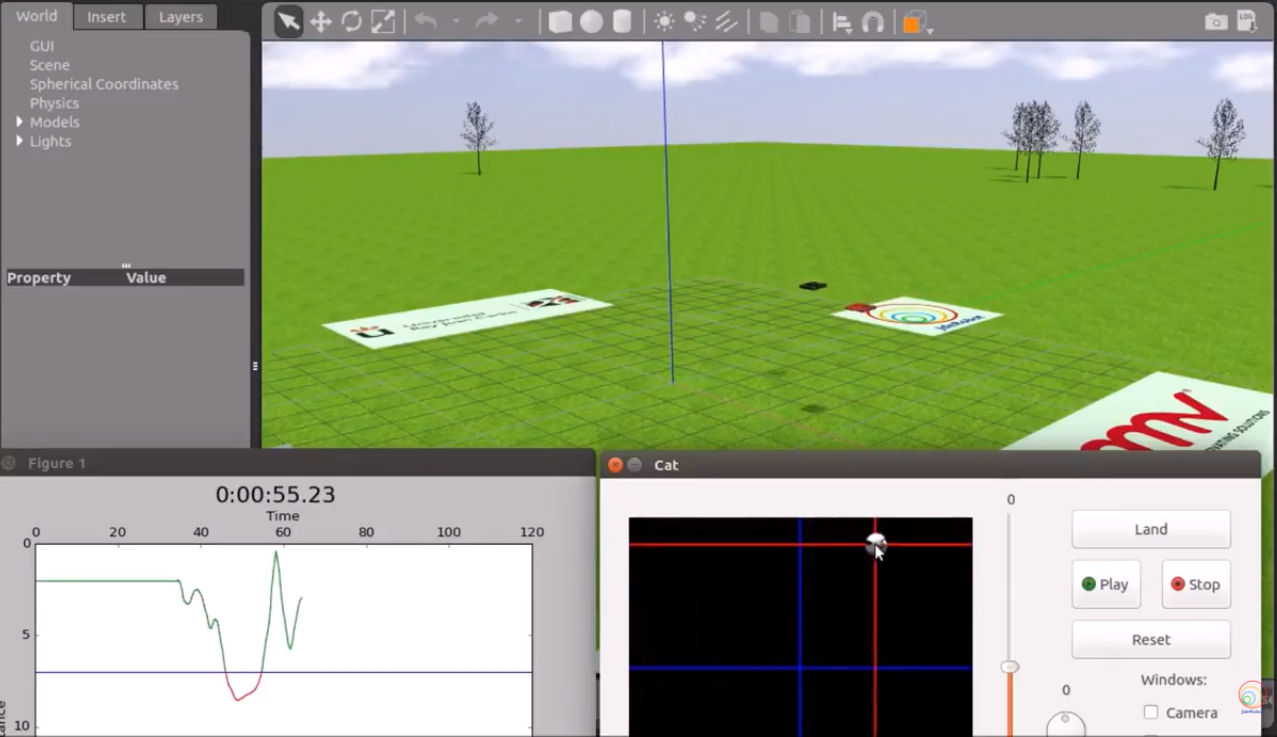
\includegraphics[width=0.95\textwidth, height=7.2cm]{figures/dronecatmouse.png}
		\caption{Drone-Cat-Mouse}
		\label{fig.dronecatmouse}
		\end{center}
\end{figure}

\textit{Drone-Cat-Mouse} es una de las prácticas más complejas del entorno JdeRobot-Academy. En ella el alumno debe dotar de la lógica necesaria a un dron (dron negro) para recoger las imágenes captadas por su cámara y filtrarlas para encontrar a un dron rojo. Una vez reconocido el dron rojo debe dotar de movimiento al dron para perseguirlo dado que el dron rojo está en movimiento. El objetivo es que el dron negro se acerque los más posible al dron rojo pero sin colisionar con él emulando el juego Gato-Ratón\footnote{\url{https://www.youtube.com/watch?v=DYD9oPawhWg}}. Esta práctica se ha utilizado en las dos ediciones del campeonato \textit{Program-A-Robot}, la primera en la URJC y la segunda en las Jornadas Nacionales de Robótica. Se va a utilzar en la tercera edición que tendrá lugar en la conferencia internacional IROS\footnote{\url{https://www.iros2018.org/competitions}}.

\subsection{Ejercicios recientes}

El contexto imediato de este Trabajo de Fin de Grado consiste en una serie de ejercicios elaborados recientemente  para enriquecer el contenido del entorno JdeRobot-Academy.

Entre los ejercicios elaborados más actuales caben destacar el TFG de Irene López Rodríguez \textit{"Nuevas Prácticas en el Entorno Docente de Robótica JdeRobot-Academy"}\cite{tfg1} en el que se introdujeron dos prácticas nuevas llamadas Coche autónomo negociando un cruce y Aspiradora autónoma con autolocalización. El primer ejercicio, después llamado \textit{Car Joint} trata sobre un coche autónomo que realiza un cruce por el que circulan coches. Para ello el coche debe filtrar las imágenes para reconocer una señal de Stop, así como los coches que circulan y las líneas de los carriles. Cuando no detecte ningún coche circulando debe tomar la intersección y escoger el carril correcto. La segunda práctica es similar a la práctica \textit{Vacuum Cleaner} pero consta del mapa con el escenario y sensor de posición, de manera que la aspiradora debe saber en qué lugar del escenario se encuentra y no repetir áreas ya limpiadas.

Otro TFG destacado en este aspecto es el de Vanessa Fernández Martínez \textit{{“Nuevas Prácticas en el Entorno Docente de Robótica JdeRobot-Academy”}}\cite{tfg2}, en el cual se añadieron dos prácticas nuevas llamadas Aspiradora Autónoma o \textit{Vacuum Cleaner} y Aparcamiento Automático, además de mejorar la práctica Tele Taxi con nuevos modelos, un mejor rendimiento del algoritmo GPP de navegación global y la inclusión de un evaluador automático capaz de medir el desempeño del algoritmo y proporcionar una nota. En cuanto al ejercicio desarrollado \textit{Vacuum Cleaner} ya ha sido comentado en el apartado anterior. La segunda práctica llamada \textit{Autopark} tiene como objetivo el aparcamiento de un coche autónomo mediante mediciones láser de los sensores frontales, laterales y posteriores.

También hay que mencionar el Trabajo de Fin de Grado desarrollado por Carlos Awadallah Estévez \textit{“Nuevas Prácticas Docentes de Robótica en el  Entorno JdeRobot-Academy”}\cite{tfg3}, en el cual se incorporan dos nuevas prácticas al entorno JdeRobot-Academy. La primera de ellas llamada \textit{Follow Face} trata de dar la lógica necesaria a una cámara pantilt de manera que procese las imágenes captadas por la cámara y reconozca la cara. Una vez hecho esto debe seguir el movimiento de la cara. La segunda práctica que se desarrolla en este TFG se llama \textit{Laser Loc} en la cual mediante mediciones de los sensores laser y un mapa con el escenario es capaz de realizar estimaciones de posición mediante movimiento y odometría.

Siguiendo con esta filosofía, el presente Trabajo de Fin de Grado aporta una práctica totalmente nueva al entorno JdeRobot-Academy y una optimización y mejora global de una práctica obsoleta incluyéndola en el entorno JdeRobot-Academy-Web.

\vspace{3cm}

El objetivo de este TFG es ampliar la variedad de prácticas que forman el entorno JdeRobot-Academy desarrollando nuevas prácticas y mejorando las exitentes para aumentar su versatilidad, además de aportar en el elenco de prácticas de JdeRobot-Academy-Web para acercar al entorno a dar soporte multiplataforma. En los próximos capítulos serán abordados los elementos necesarios para conseguir este objetivo. Comenzaremos con el Capítulo 2, en el que se concretarán los objetivos marcados, así como el punto de partida de este TFG y la metodología que ha sido empleada. En la Capítulo 3 se abordará la infraestructura utilizada para realizar el proyecto. En los Capítulos 4 y 5 explicaremos las prácticas que se han abordado en este TFG. Y, por último, en el Capítulo 6, se expondrán las conclusiones obtenidas, además de las posibles líneas de mejora futuras.


\lhead[]{CAP\'ITULO \thechapter. OBJETIVOS}
\chapter{Objetivos}\label{cap.objetivos}
Una vez introducido el contexto en que se ha desarrollado este trabajo, es hora de profundizar en los objetivos que se han tratado de alcanzar, los requisistos para las soluciones desarrolladas y la metodología que se ha seguido para conseguirlos.

\section{Objetivos}
La meta alcanzada en este preyecto es el desarrollo de una nueva práctica de sisemas robóticos para el entorno docente de JdeRobot-Academy llamada \textit{Chrono} y la optimización de una práctica existente llamada \textit{Follow Road}, así como una actualización de sus drivers para que soporte ROS y su inclusión en la infraestructura web de JdeRobot-Academy-Web.

La primera práctica consiste en la competición de dos coches de F1 por un circuito que dispone de una línea roja que se debe seguir. El código del alumno competirá con el F1 del mejor tiempo registrado para el circuito en el que esté compitiendo. De esta manera consguiremos que el alumno pueda depurar su código de solución y tenga un estímulo para alncanzar la perfección en el desarrollo de su algoritmo.

En cuanto a la segunda práctica, trata de un dron con con una cámara que debe seguir una carretera. El código del alumno deberá filtrar las imágenes para segmentar la carretera y dotar de un movimiento conttrolado al dron que le permita seguir la carretera.

\section{Requisitos}
A continuación se van a enumerar los requisitos necesarios para proporcionar soporte al software desarrollado:

\begin{enumerate}
	\item El Sistema Operativo empleado será Ubuntu 16.04 LTS.
	\item Se utilizará el \textit{middleware} robótico JdeRobot en su versión 5.6.2. El uso de este \textit{middleware} robótico simplifica el desarrollo del comportamiento del robot.
	\item Se usará \textit{OpenCV3} para la filtración de las imágenes captadas por las cámaras en ambas prácticas.
	\item Para dar soporte a los sensores y actuadores se utilizará \textit{ROS-Kinetic}.
	\item Para mostrar el comportamiento de los robots y el desarrollo de un mundo que los soporte se utilizará el simulador \textit{Gazebo}.
	\item El lenguaje de programación utilizado para el desarollo de ambas prácticas será \textit{Python} en su versión 2.7.12, por compatibilidad con el \textit{middleware} robótico JdeRobot y con el \textit{middleware ROS-Kinetic}.
	\item Las soluciones desarrolladas deben ejecutar algoritmos en tiempo real, por lo que deben ser eficientes y realizar movimientos suaves.
\end{enumerate}

\section{Metodología}
El desarrollo de este Trabajo de Fin de Grado puede descomponerse en un conjunto de iteraciones con distintas fase. Cada fase está formada por una reunión semanal con el tutor para determinar los objetivos a abordar, la planificación de cómo abordarlos, intentar solucionar los problemas que vayan a surgir anticipadamente y la consecución de los objetivos durante la semana. De esta manera se ha coneguido un desarrollo fluido y completo, asentando los conocimientos y despejando las dudas que surgían durante los meses dedicados a este deesarrollo.

Además de las reuniones semanales, se han utilizado herramientas de apoyo como la bitácora semanal en la Wiki de JdeRobot\footnote{\url{https://jderobot.org/Pablomoreno-tfg}}, donde se redactaban los avances obtenidos acompañados de vídeos demostrativos e imágenes. El código desarrollado se almacenaba, progresivamente, en la plataforma Github, en un repositorio personal\footnote{\url{https://github.com/RoboticsURJC-students/2017-tfg-pablo-moreno}} \footnote{\url{https://github.com/PabloMorenoVera/JdeRobot}} \footnote{\url{https://github.com/PabloMorenoVera/Academy}}, a los cuales el tutor tiene acceso para dar realimentación y orientar el proceso.

 El modelo de desarrollo escogido ha sido el modelo creado por Barry Boehm, dado que al tratarse de un modelo en espiral, se adaptada a la perfección a nuestras necesidades, permitiendo disponer de flexibilidad ante cambios en los requisitos semanales, algo común mientras avanzaba el desarrollo, a la par que nos permitía separar el objetivo final en varias sub-tareas más sencillas. Con esto se ha conseguido una subsanación de los riesgos temprana y la definición de una arquitectura en las fases iniciales del desarrollo, todo ello dotado con un control de calidad continuo.

\begin{figure}[H]
  \begin{center}
    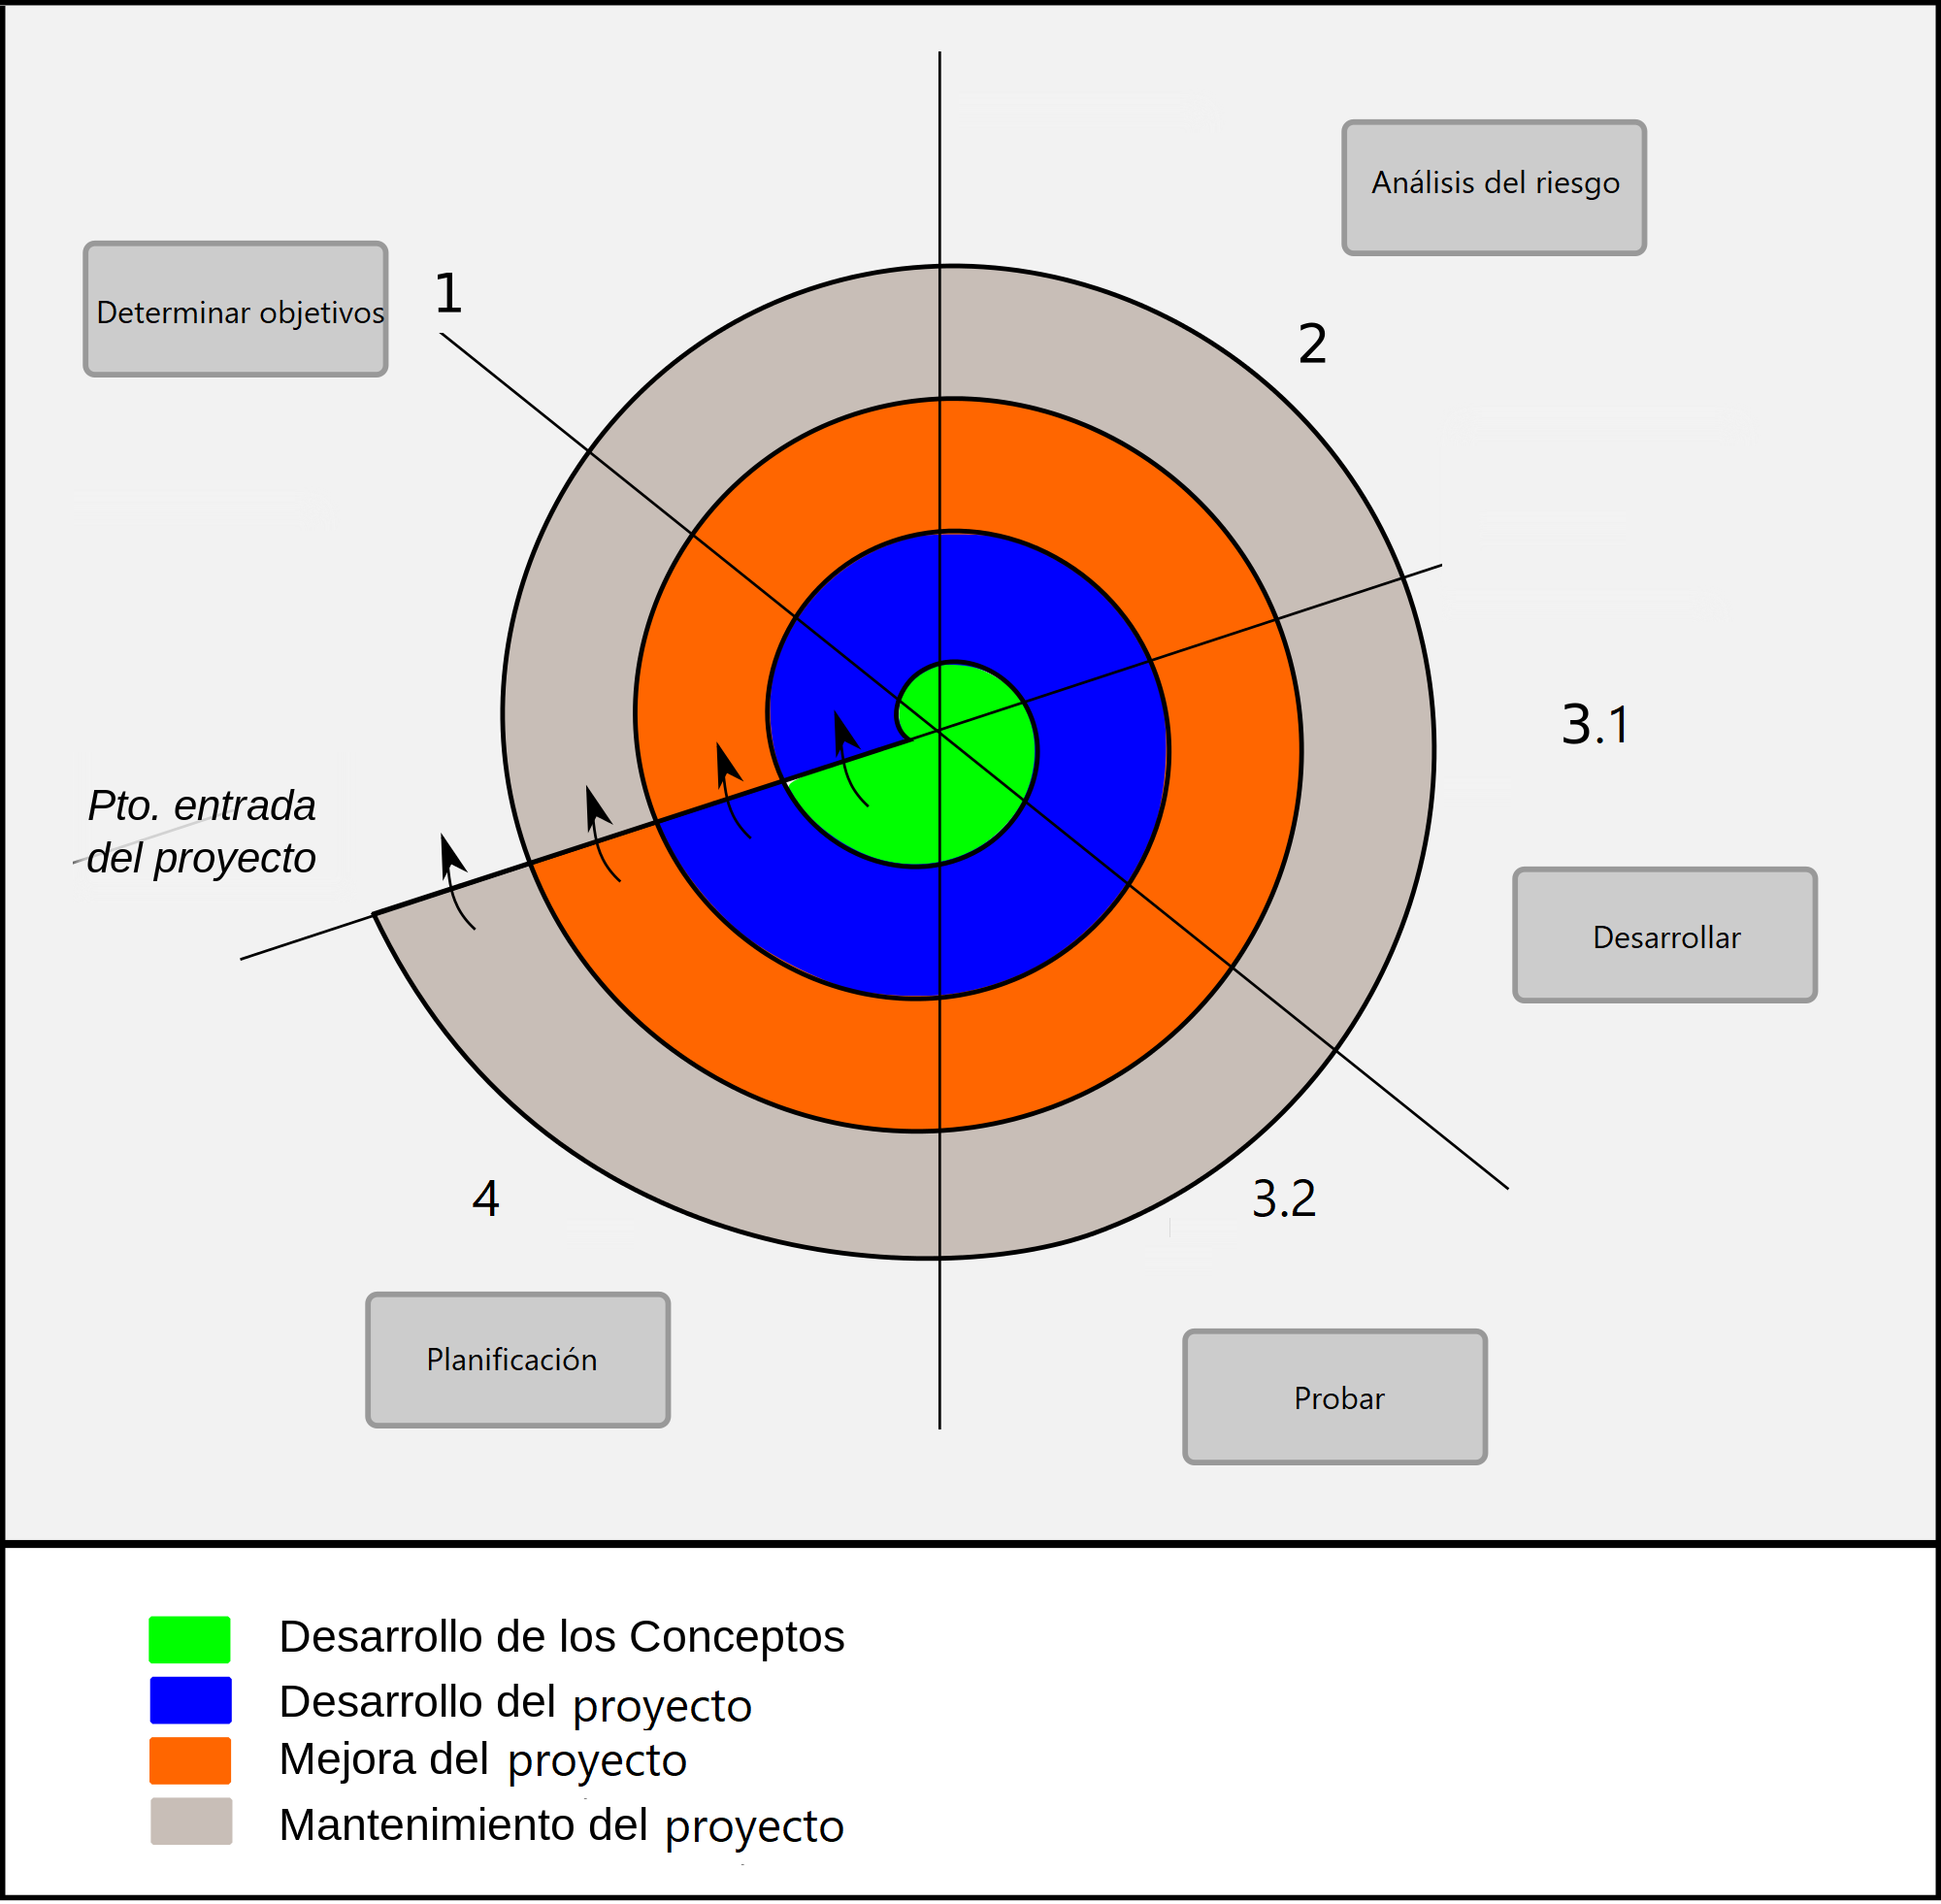
\includegraphics[width=0.9\linewidth]{figures/modelo_espiral.png}
		\caption{Modelo de desarrollo en espiral}
		\label{fig.espiral}
		\end{center}
\end{figure}

La ventaja de este ciclo de vida es que permite la obtenicón de prototipos funcionales en una etapa temprana, la optimización progresiva del prototipo desarrollado y, en última instancia, pulir los detalles para abarcar la totalidad de los requisitos especificados (Figura 2.1). De esta manera el trabajo se desarrolla de manera incremental con cuatro fases bien definidas:

\begin{itemize}
	\item[--] \textbf{Determinar objetivos}: Esta primera fase del ciclo está formada por la definición de las metas.
	\item[--] \textbf{Análisis del riesgo}: Se evalúan los posibles problemas iniciales al desarrollo y las soluciones a los mismos.
	\item[--] \textbf{Desarrollar y probar}: En esta tercera fase se procede al desarrollo del trabajo propiamente dicho, junto con una serie de pruebas para verificar su funcionamiento.
	\item[--] \textbf{Planificación}: En esta última fase del ciclo se valoran los resultados obtenidos y se planifican las siguientes etapas del proyecto.
\end{itemize}

\section{Plan de trabajo}
Para la consecución de los objetivos descritos, se han seguido las siguientes etapas de trabajo:

\begin{itemize}
	\item[--] \textbf{Familiarización con el entorno JdeRobot}: una vez descargado e instalado tanto el software, dependencias y bibliotecas como el simulador, se tomará un primer contacto con el entorno JdeRobot mediante la modificación y readaptación de algunas prácticas existentes, como sus interfaces gráficas.
	\item[--] \textbf{Toma de contacto con el simulador Gazebo}: esa etapa se ha dedicado al desarrollo de algunos modelos en el simmulador, estudiando ejemplos disponibles en la web\footnote{\url{http://gazebosim.org/tutorials}} y en JdeRobot, así como modificándolos y desarrollando algunos modelos nuevos (Figuras ~\ref{fig:estanteria} y ~\ref{fig:warehouserobot}). En esta etapa también se han estudiado el funcionamiento básico de los \textit{plugins} que dispone Gazebo para el control de sus robots, sensores y acutadores. Esto ha suspuesto una toma de contacto con el lenguaje de programación C++ utilizado, también, para comprender los \textit{plugins} de ROS-Kinetic.
\begin{figure}[H]
	\centering
	\begin{minipage}[h]{.48\linewidth}
		\centering
		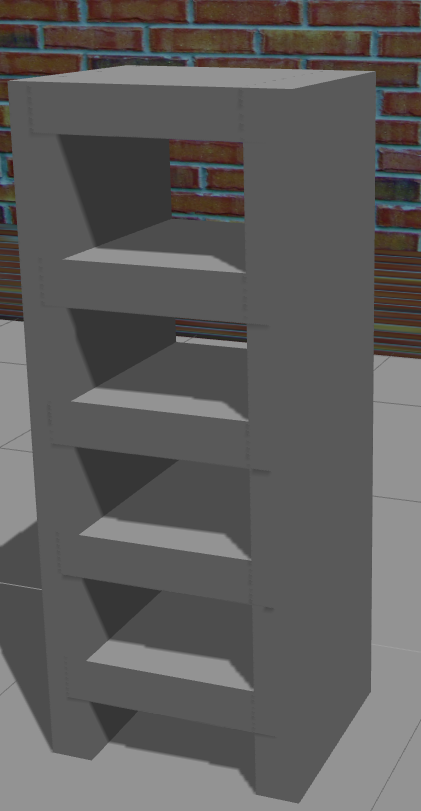
\includegraphics[width=.5\linewidth, height=7cm]{figures/estanteria.png}
		\captionof{figure}{Modelo estantería}
		\label{fig:estanteria}
	\end{minipage}
	\begin{minipage}[H]{.48\linewidth}
		\centering
		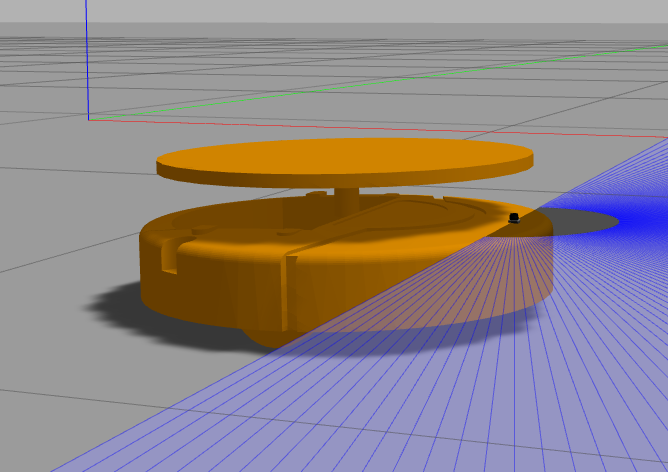
\includegraphics[width=.7\linewidth, height=7cm]{figures/warehouse_robot.png}
		\captionof{figure}{Warehouse robot}
		\label{fig:warehouserobot}
	\end{minipage}
\end{figure}
	\item[--] \textbf{Estudio de las bibliotecas}: En este punto fue necesario el estudio de diferentes bibliotecas disponibles en python para poder comenzar con el desarrollo de las prácticas. Fue necesario el estudio de bibliotecas como \textit{OpenCV}, Threading, Numpy y PyQt5.
	\item[--] \textbf{Optimización de la práctica del sigue carretera}: Esta práctica estaba bastante obsoleta y se procedió a renovar por completo su interfaz gráfica, el escenario utilizado incluyendo un nuevo dron que soportaba ROS y una nueva conexión de los sensores y actuadores del propio dron. Además se desarrolló una optimización global del nodo académico como la inclusión de una pausa académica. Además se creó una versión de la práctica para la plataforma Jupyter y se incluyó en el elenco de práticas soportadas en JdeRobot-Academy-Web.
	\item[--] \textbf{Desarrollo de una solución de referencia para la práctica}.
	\item[--] \textbf{Preparación de la infraestuctura del ejercicio chrono}: Se desarrollará el modelo del F1 y el circuito para competir en \textit{Blender} y \textit{SketchUp} para conformar el escenario de Gazebo. También se desarrollarán los drivers del robot F1 para dar soporte en ROS-Kinetic de los motores. la cámara y el láser. Se creará el noodo académico de la práctica para alojar el código del estudiante y la versión de la práctica para Jupyter.
	\item[--] \textbf{Desarrollo de una solución de referencia para chrono}.
\end{itemize}
\lhead[]{CAP\'ITULO \thechapter. INFRAESTRUCTURA}
\chapter{Infraestructura}\label{cap.infraestructura}
En este capítulo tratará de abordar todos los componentes y software que han servido de apoyo en el desarrollo del TFG. En este punto daremos una explicación detallada sobre las plataformas en las que se cimienta el trabajo (ROS y JdeRobot), en el simulador Gazebo, en los editores de modelos, en las librerías más importantes (OpenCV y PyQt), en el proyecto Jupyter y en el entorno JdeRobot-Academy-Web.

\section{Entorno ROS}
ROS (Robot Operating System) proporciona a los desarrolladores de software robótico los componentes necesarios para el desarrollo de aplicaciones robóticas. Entre ellos destacan la abstracción hardware, bibliotecas, intercambios de mensajes, administración de paquetes, controladores de dispositivo y visualizadores. Esta plataforma se distribuye en código abierto bajo una licencia BSD.

Una de las características más importantes de ROS es su integración con el simulador Gazebo, con el que se comunica a través de paquetes llamados \textit{gazebo\_ros\_pkgs} \footnote{\url{http://ros.org/wiki/gazebo\_ros\_pkgs}}. Mediante estos paquetes, ROS es capaz de proporcionar las interfaces necesarias para simular un robot en Gazebo usando \textit{ROS Messages}, servicios y reconfiguración mecánica.

Esta plataforma se conforma como una colección de nodos o procesos que suponen una computación. Los nodos se combinan en un gráfico y se comunican entre sí mediante \textit{topics} de transmisión, servicios RPC y el Servidor de Parámetros. Un sistema de control de un robot se formará por la integración de distintos nodos, cuanto mayor sea la funcionalidad de la que se dote al robo, mayor número de nodos tendrá. Existen nodos de control de láser, vista gráfica del sistema, motores de ruedas, odometría, cámaras, etc. La existencia de nodos de ROS en el robot proporciona beneficios para el sistema robótico como tolerancia adicional a fallos soportados por cada nodo de manera indivual, de esta manera el fallo se concentra en un solo nodo. Además, la complejidad del código se reduce con los sistemas monolíticos.

Los \textit{topics} de ROS actúan como forma de comunicación, de esta manera se definen como buses sobre los que los nodos intercambian mensajes. Gracias a la semántica de publicación y/o suscripción anónima de los \textit{topics}, se desacopla la producción de información de consumo. Debido a esto los nodos no saben con quién se están comunicando. Por otra parte, los nodos interesados en un \textit{topic}, se suscriben a él para recoger la información que se publique por el mismo y, por otra parte, los nodos que generen datos pertenecientes a ese \textit{topic}, transmitirán la información por él. Es importante destacar que puede haber varios editores o generadores y varios suscriptores del mismo \textit{topic}.

Debido a la compatibilidad de ROS con Gazebo y con JdeRobot, se pueden utilizar los \textit{plugins} de ROS para las simulaciones en Gazebo de las prácticas presentes en el entorno JdeRobot mediante el establecimiento de las conexiones de los sensores y actuadores de la práctica con los \textit{plugins} de ROS en el nodo académico de la misma.

Existen una gran cantidad de \textit{plugins} de ROS que proporcionan una enorme diversidad de funcionalidad para el desarrollo de robots \footnote{\url{http://wiki.ros.org/gazebo_plugins}}. Entre ellos destacan el plugin que controla el láser, llamado \textit{libgazebo\_ros\_laser} o el que controla una cámara, llamado \textit{libgazebo\_ros\_camera}. Ambos plugins serán usados en las prácticas contenidas en este Trabajo de Fin de Grado.

\section{JdeRobot}
La plataforma \textit{JdeRobot}\footnote{\url{http://jderobot.org}} es un \textit{middleware} abierto para desarrolladores de robots y visión artificial. Fue creada por el Grupo de Robótica de la Universidad Rey Juan Carlos en 2003 y está licenciada como GPLv3\footnote{\url{https://www.gnu.org/licenses/quick-guide-gplv3.html}}.
La estructura de esta plataforma ha sido desarrollada en C y C++, aunque tiene componentes escritos en Python y JavaScript. El entorno ofrecido es mediante componentes, los cuales son ejecutados como procesos que interoperan entre sí mediante \textit{middleware} de comunicaciones como ICE o \textit{ROS-Messages}, que permiten la interoperación de componente en un entorno multilenguaje.

JdeRobot facilita los \textit{drivers} necesarios para la funcionalidad de sus robots. De esta manera, los \textit{dirvers} están asociados al hardware del robot proporcionando interfaces de acceso, por lo que simplifica la comunicación de las aplicaciones con los actuadores del robot que se realiza mediante una función mediante los interfaces ICE o ROS.

Los dispositivos que se pueden encontrar en JdeRobot son muy diversos, destacan el cuadricópteros como el Ardronde de Parrot, operativo con ICE, o el SoloDrone de 3DR, operativo con ROS, los coches Fórmula1 desarrollados por la propia plataforma JdeRobot que incluyen modelos de la mayoría de las escuderías presentes en la Fórmula 1, operativos con ROS y modificados en este TFG para incluirlos en la plataforma. También se incluyen modelos como el boto Kobuki de Yujin Robot, el humanoide NAO de Aldebaran Robotics, cámaras fireware, USB e IP, los simuladores Stage y Gazebo, escáneres láser LMS de SICK y URG de Hokuyo, sensores de profundidad como Kinect y otros dispositivos X10 de domótica o \textit{drivers} específicos de control de cámaras, láser y motores de movimiento.

JdeRobot incorpora librerías de software libre para su uso como OpenCV para visión, Eligen para álgebra o PCL para manejo de nubes de puntos. Al ser compatible con ROS, en específico con ROS-Kinetic, las aplicaciones de la plataforma pueden incorporar nodos de ROS y conectarse a ellos de manera fluida.

Las prácticas que componen este Trabajo de Fin de Grado se han desarrollado en la versión de JdeRobot 5.6.2, última versión estable.

\section{Simulador Gazebo}
Gazebo\footnote{\url{http://gazebosim.org/}} es un simulador de robótica que permite emular escenarios tridimensionales para robots autónomos (Figura 3.1). Es apropiado para comprobar algoritmos basados en visión artificial y elusión de objetos. Al desarrollar algoritmos de control de robots es necesaria la realización de pruebas del software para confirmar la validez del código escrito. Es por ello que Gazebo adquiere una gran importancia como simulador, dado que permite probar la eficacia del código sin necesidad de probarlo con hardware real, pudiendo dañarlo. De esta manera los simuladores son importantes en la robótica, dado que permiten abaratar costes evitando los daños en el hardware del robot.

El simulador utilizado en el presente Trabajo de Fin de Grado es Gazebo, al ser de código abierto, versátil (capaz de simular objetos, robots y sensores en entornos complejos de interior y exterior), al posees una interfaz de gran calidad y un robusto motor de físicas (pueden describirse componentes como la masa, rozamientos, inercia, amortiguamiento, etc.). Fue elegido para soportar el DARPA Robotics Challenge de 2012 a 2015 y está mantenido por la Fundación Open Robotics\footnote{\url{https://www.openrobotics.org/}}

\begin{figure}[H]
  \begin{center}
    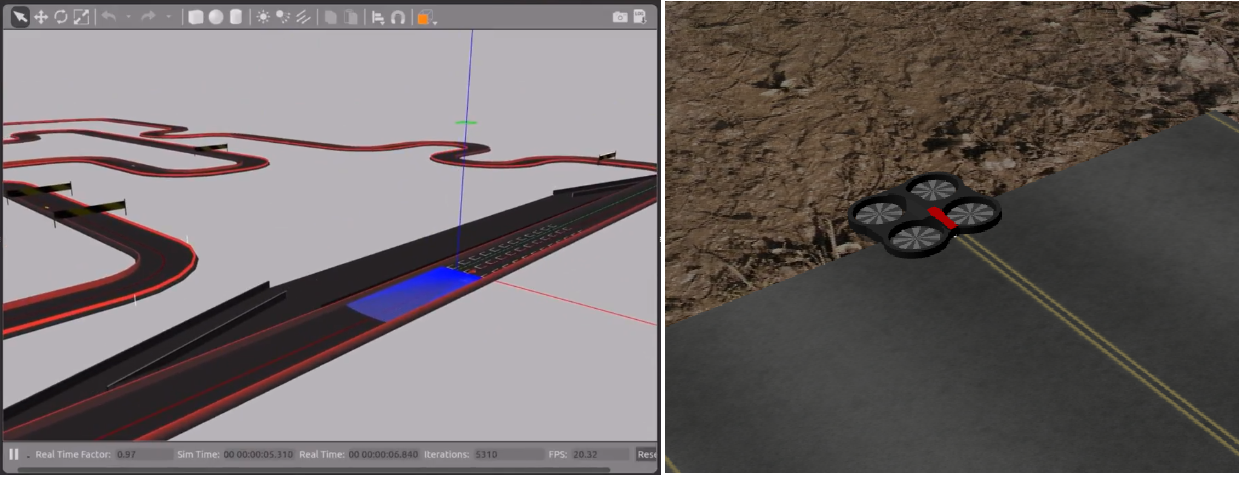
\includegraphics[width=0.9\linewidth]{figures/gazeboworlds.png}
		\caption{Ejemplo de mundo y modelo de Gazebo}
		\label{fig.worlds}
		\end{center}
\end{figure}

Los escenarios de Gazebo se describen en fichero con extensión ".world", que son ficheros escritos en XML (Extensible Remarkable Language) de descripción de documentos, definidos en el lenguaje de simulación SDF (Simulation Description Format), donde se recogen todos los elementos del escenario:

\begin{itemize}
	\item Escena: Iluminación, propiedades del cielo, sombras, etc.
	\item Mundo: Representación del mundo como conjunto de modelos, \textit{plugins} y propiedades físicas.
	\item Modelo: Componentes que forman el robot, como articulaciones, objetos de colisión, sensores, etc.
	\item Físicas: Gravedad, inercia, rozamiento, colisiones, motor físico, tiempo, etc.
	\item \textit{Plugins}: Pueden incluirse en el mundo, el modelo o un sensor. Pueden incluirse \textit{plugins} disponibles en la red como el que da soporte completo a la funcionalidad del robot Roomba, llamado \textit{libroombaplugin.so}.
\end{itemize}

Cada elemento del escenario cuenta con una etiqueta propia que lo distingue del resto. Cualquier propiedad descrita dentro de su etiqueta tiene que ir marcada con la etiquete de la propiedad correspondiente.
En la versión 7 de Gazebo se ha incluido un editor de modelos básico para poder desarrollar modelos y escenarios básicos. A partir de los modelos que se importen o desarrollen en Gazebo, es necesario adjuntar un \textit{plugin} que los dote de la funcionalidad necesaria, de otra manera no serían más que simples objetos inanimados.

\section{Editor de modelos}
Para el desarrollo del modelo de robots se ha trabajo con dos editores de modelos, SketchUp\footnote{\url{https://www.sketchup.com/}} y Blender\footnote{\url{https://www.blender.org/}}. Estos editores son necesarios para importar los modelos de robots generados en ellos al simulador Gazebo.
Existe un almacén web desde donde es posible descargarse una gran variedad de modelos y escenarios, además de desarrollar los propios. Una vez desarrollado el modelo o escenario, estos editores exportan el modelo o escenario en formato ".dae" (Digital Assets Exchange), formato perteneciente al lenguaje XML, y los correspondientes texturas en imágenes con formato ".JPG". Una vez obtenidos estos ficheros, ya son importables por el simulador Gazebo, pero es necesario una modificación para dotar al modelo o escenario de colisiones, inercias, gravedad, etc. 

Los escenarios y modelos generados por estos editores son creados mediante la intersección de líneas, generando los distintos tipos de objetos. Además, es posible adjuntar una textura o color a cada cara que forma el objeto. Además, el editor Blender, al ser más complejo, permite la introducción de iluminación y trabajar con formas geométricas en tres dimensiones directamente, en cambio el editor SketchUp trabaja con líneas, aunque es más sencillo de utilizar.

El editor de modelos Blender es de código abierto pero el editor de modelos SketchUp es de pago, pero tiene la ventaja de contar con su almacén de modelos en el que puedes descargar una gran variedad de modelos.

\section{Lenguaje Python}
Python\footnote{\url{https://www.python.org/}} es un lenguaje de programación orientado a objetos, interpretado y de alto nivel con semántica dinámica. Es un lenguaje de fácil aprendizaje y comprensión debido a su apariencia intuitiva. Su creador fue Guido van Rossum, un investigador holandés que trabajaba en el centro de investigación CWI (Centrum Wiskunde \& Informática. La primera versión de este lenguaje de programación surgió en 1991, pero no fue publicado hasta tres años después. El nombre que recibió este lenguaje fue dado por su creador en honor a la serie de televisión \textit{Monty Python's Flying Circus}.

La combinación del tipado y el enlace dinámico con sus estructuras de datos integradas de alto nivel, dotan a este lenguaje de un desarrollo rápido de aplicaciones, scripting o lenguaje de interconexión de componentes existentes. La sintaxis fácil y simple enfatiza su legibilidad y reduce el coste de mantenimiento del código. Además, Python admite módulos y paquetes, por lo que fomenta la modularidad del programa y la reutilización de código.

El intérprete de Python y la extensa biblioteca de paquetes están disponibles en formato binario o en código fuente de manera gratuita para las plataformas principales y pueden ser distribuidas libremente.

La última versión de Python Software Fundation es la 3.6.5. En este Trabajo de Fin de Grado hemos utilizado la versión 2.7.12, compatible con JdeRobot 5.6.2 y con ROS-Kinetic. De manera que la completitud de las dos prácticas desarrolladas en este trabajo está escrita en esta versión.

\section{Biblioteca OpenCV}
OpenCV\footnote{\url{https://opencv.org/}} (Open Source Computer Vision Library) es una librería de código abierto destinada al procesamiento de imágenes y el aprendizaje máquina. Fue desarrollada por Intel y publicada bajo licencia de BSD. El propósito de esta librería es facilitar el desarrollo de programas de visión por computador en tiempo real.

Se trata de una librería multiplataforma con soporte para MacOS, Linux, Android y Windows. Además, existen versiones en Java, Python y C\# a pesar de que era, originalmente, una librería en C/C++. También existen interfaces en desarrollo para Ruby, Matlab y otros lenguajes.
La librería OpenCV implementa algoritmos para técnicas de detección de rasgos, clasificación de acciones humanas en vídeos, reconocimiento, segmentación de objetos, calibración, seguimiento de caras, análisis de la forma y movimiento, reconstrucción 3D... Los algoritmo que componen esta librería están basados en estructuras de datos flexibles acoplados a estructuras IPL (\textit{Intel Image Processing Library}), utilizando la arquitectura de Intel respecto a la optimzación de la mayoría del paquete. También aprovecha la aceleración de cómputo gracias al uso de tarjetas gráficas avanzadas (GPUs). OpenCV fue desarrollado para tener una alta eficiencia computacional. Está escrito en el lenguaje de programación C y puede aprovechar las ventajas de los procesadores \textit{multicore} de nueva generación. Tales son las ventajas que aporta que las grandes compañías como Google, Yahoo, Microsoft, Intel, IBM, Sony, Toyota u Honda utilizan esta librería, que se ha convertido en el estándar de facto en su campo.

Para este trabajo se ha utilizado la librería OpenCV en la versión 3.2 y su ha sido empleada en toda la parte del código relacionada con tratamiento de imágenes.

\section{Biblioteca PyQt}
PyQt\footnote{\url{https://pypi.org/project/PyQt5/}} es un conjunto de enlaces Python utilizado para el conjunto de herramientas Qt, un \textit{framework} multiplataforma orientado a objetos y escrito en C++ que permite el desarrollo de interfaces gráficas. Incluye sockets, hilos, bases de datos SQL, Unicode, etc. Combina todas las ventajas de Qt y Python empleando todas las funcionalidades de Qt con un lenguaje de programación sencillo como es Python. Fue desarrollada por Riverbank Computing Ltd y tiene suporte multiplataforma con versiones para Windows, Linux, Mac OS X, iOS y Android.

Para este proyecto se ha utilizado la versión 5 de PyQt. Se trata de un conjunto de enlaces Python para Qt5, con soporte para Python 2.x y Python 3.x. Incluye más de 6000 funciones y 620 clases y métodos. Dispone de una licencia dual, es decir, puede elegirse una licencia comercial para usuarios o una licencia GPL (General Public Licence) para desarrolladores.
Las clases de PyQt5 se dividen en módulos: QtCore, QtGui, QtWidgets, QtXml y QtSql, entre otros. Para las prácticas desarrolladas, se han utilizado los siguientes módulos:
\begin{itemize}
	\item QtGui: contiene clases para la creación de interfaces gráficas y el desarrollo de gráficos en 2D, imágenes, texto y desarrollo de ventanas.
	\item QtCore: incorpora las clases principales no relacionadas con la interfaz gráfica. Se utiliza para trabajar con archivos, hilos, datos, procesos, urls, etc.
	\item QtWidgets: está formado por clases que proporcionan distintas funcionalidades a la interfaz del usuario.
\end{itemize}

\section{Jupyter}
Jupyter Notebook\footnote{\url{http://jupyter.org/}} se trata de una aplicación web de código abierto que permite al usuario desarrollar y compartir documentos que contengan código empotrado, ecuaciones, textos y visualizaciones. Proporciona una gran variedad de ventajas entre las que destacan limpieza, simulación numérica, modelado estadístico, visualización y transformación de datos, aprendizaje automático, etc. Inicialmente fue desarrollado como IPython 3.0 pero se renombró como Jupyter.

El cuadernillo de trabajo o \textit{Notebook} está compuesto por celdas en las que se inserta el código, en lenguaje Python, o distintos elementos de texto enriquecido como párrafos, ecuaciones, enlaces, figuras, etc. El resto de tipos de celdas son legibles para los humanos como figuras, tablas o texto y contienen los análisis y resultados del trabajo, además de documentos ejecutables para la ejecución del análisis.
El \textit{Notebook} está formado por una sucesión lineal de celdas. Hay cuatro tipos básicos:

\begin{itemize}
	\item \textbf{Celda de código}: se trata de input y output de código que se ejecuta en el kernel del cuadernillo a tiempo real.
	\item \textbf{Casillas de reducción}: son celdas de texto con ecuaciones en LaTex empotradas.
	\item \textbf{Encabezado de celdas}: formado por 6 niveles de organización jerárquica y su formato.
	\item \textbf{Celdas sin formato}: se trata de texto sin formato que se incluye en el cuadernillo sin ningún tipo de modificación cuando los cuadernillos son convertidos a formatos distintos mediante \textit{nbconvert}.
\end{itemize}

La aplicación tiene un modelo cliente-servidor que permite la ejecución y edición de los \textit{Notebooks} mediante un navegador web. La aplicación Jupyter puede ejecutarse desde un escritorio local sin necesidad de disponer de conexión a Internet o instalarse en un servidor remoto y acceder a ella a través de internet. Además de estas características, Jupyter dispone de un \textit{Panel de control} o llamado \textit{Dashboard} con el que permite la apertura, guardado y cierre de los archivos y los núcleos del \textit{Kernel}.

Estos \textit{kernels} son motores computacionales que ejecutan el código contenido en el \textit{Notebook}. Existen multitud de \textit{kernels} oficiales que dan soporte a distintos lenguajes como Python, Julia, R, Ruby Haskell, Scala, ...), incluso versiones distintas de \textit{kernels} para un mismo lenguaje. Al abrir el \textit{Notebook}, el \textit{kernel} se inicializa automáticamente. De este modo, al ejecutar una celda del cuadernillo se reproduce el código contenido en ella y, a continuación, de muestran los resultados. Es importante tener en cuenta que, dependiendo del código contenido en la celda, el \textit{kernel} puede consumir una gran cantidad de recursos CPU y RAM, que están limitados por el navegador.

Los cuadernillos, así como el resto de tipos de documentos (ficheros de código auxiliar, fichero de texto, imágenes, etc.) pueden guardarse y son almacenados en el sistema de fichero local del usuario. El \textit{Notebook} será almacenado con una extensión \textit{.ipynb} que puede ser ejecutado tras iniciar Jupyter.

Gracias a esta aplicación, se han desarrollado prácticas análogas a las existentes en la plataforma \textit{JdeRobot-Academy} en Jupyter. De esta manera, JdeRobot se acerca a dar soporte multiplataforma gracias al uso del navegador web y Jupyter para la interacción con su entorno docente. Para ello se ha empotrado el nodo académico de las prácticas en celdillas de un \textit{Noteboook} de Jupyter y se ha proporcionado una celdilla para que el alumno escriba el algoritmo de solución en él y sólo tenga que ejecutar esa celdilla para ver los resultados.
Los \textit{Notebooks} utilizados para la recreación de las prácticas han sido desarrollados en la versión 2.7 de Python, por lo que las prácticas y la solución que desarrollen los alumnos deben ser en esta versión.

\section{Academy-Web}
Esta plataforma web proporciona un servidor remoto para el desarrollo y ejecución de las prácticas contenidas en el entorno \textit{JdeRobot-Academy}. Esto supone una gran innovación y el paso final al soporte multiplataforma del entorno docente \textit{JdeRobot}.

Para ello se basa en el uso de Jupyter para cargar el nodo académico de las prácticas, así como de un script (incluido en el \textit{Notebook} de Jupyter) para realizar las conexiones de los sensores y actuadores del robot con el nodo académico. También utiliza el soporte del simulador Gazebo en navegadores web para ofrecer una visualización del escenario de la práctica cargando un fichero \textit{.world} donde se incluye la descripción del robot y el mundo. Para soportar esta carga computacional, el servidor de la plataforma está basado en el servidor \textit{Apache}\footnote{\url{https://www.apache.org/}}, sobre el que se ha desarrollado un servidor en  \textit{Django}\footnote{\url{https://www.djangoproject.com/}}. Ambas plataformas son de código libre y proporcionan el código necesario para el desarrollo de servidores web. Por último, utiliza \textit{Dockers}\footnote{\url{https://www.docker.com/}} para ofrecer al estudiante todos los componentes necesarios para dar soporte a toda la infraestructura anterior. De esta manera, tanto JdeRobot, ROS-Kinetic, modelos, escenarios, \textit{plugins}, \textit{drivers}, etc. Están disponibles y son totalmente transparentes al alumno.

Mediante la integración de todas las plataformas anteriores se ha conseguido desarrollar el servidor web \textit{Academy-Web} que proporciona al estudiante todas las herramientas necesarias para realizar las prácticas que contiene en cualquier plataforma de una manera muy sencilla. el servidor ofrece la visualización del escenario en Gazebo junto con el cuadernillo de Jupyter en el que está presente la celda en la que el estudiante desarrollará su código (Figura 3.2).

\begin{figure}[H]
  \begin{center}
    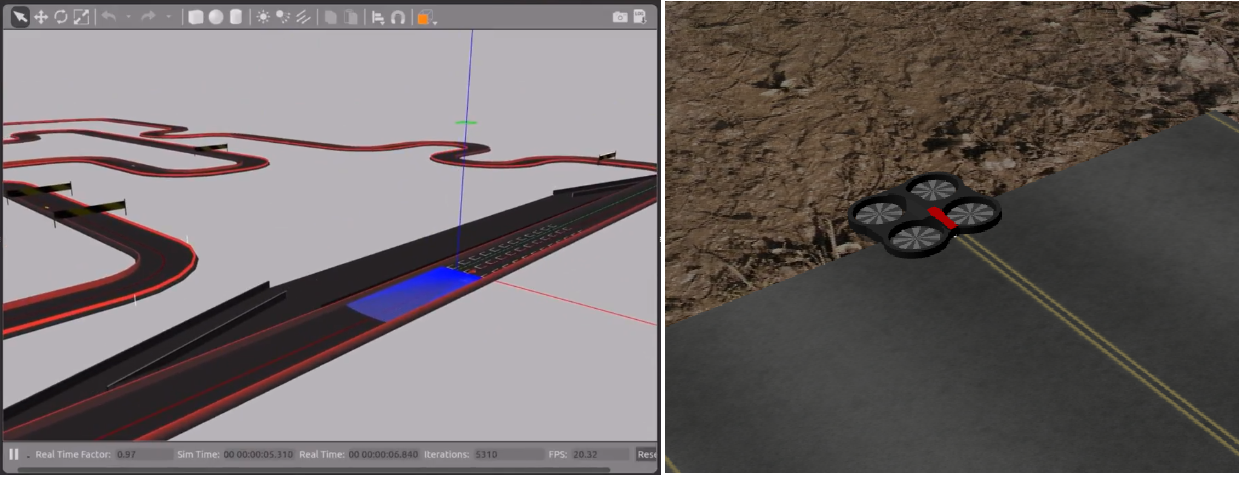
\includegraphics[width=0.9\linewidth]{figures/gazeboworlds.png}
		\caption{Visualización de la práctica XXXXX en Academy-Web}
		\label{fig.academyweb}
		\end{center}
\end{figure}


%\lhead[]{CAP\'ITULO \thechapter. FOLLOW FACE}
%\include{4-FollowFace}
%\lhead[]{CAP\'ITULO \thechapter. LASER LOC}
%\include{5-LaserLoc}
\lhead[]{CAP\'ITULO \thechapter. CONCLUSIONES}
\chapter{Conclusiones}\label{cap.conclusiones}
Una vez documentadas en profundidad las dos prácticas desarrolladas en este Trabajo de Fin de Grado, se dedicará el siguiente capítulo a la comprobación de la consecución de los objetivos alcanzados, así como a la explicación de los conocimientos adquiridos y una breve exposición de posibles mejoras de las prácticas y de las líneas de actuación futuras.

\section{Conclusiones}
El objetivo principal de desarrollar una nueva práctica y la consecución de una mejora notoria en otra de las prácticas del entorno JdeRbot-Academy ha sido alcanzado con éxito. Prueba de ello son, tanto su inclusión en el programa de prácticas, como el correcto funcionamiento del nodo académico y de la solución de referencia desarrollada. Este objetivo principal estaba subdividido en objetivos secundarios de los cuales se detallará a continuación si han sido alcanzado y la manera para ello.

El primer objetivo secundario establecido fue la mejora de una práctica existente del entorno de JdeRobot-Academy. La práctica escogida fue el sigue carreteras o \textit{Follow Road}. Este objetivo se logró alcanzar dado que la práctica fue completamente optimizada y mejorada. Se desarrollaron mejoras en la interfaz gráfica y el nodo académico, como la introducción de un visor de imágenes filtradas y el desarrollo de una pausa académica. Además, se realizó una optimización de la práctica incluyendo \textit{drivers} de ROS para der un mejor soporte a su infraestructura. De esta manera se tuvo que hacer una readaptación de las conexiones del nodo académico con sensores y actuadores del robot. Después de todas estas modificaciones se consiguió una práctica totalmente operativa y actualizada. Tanto es así, que la renovación de la interfaz gráfica se incluyó en las prácticas similares del entorno JdeRobot-Academy.

El siguiente objetivo fue el desarrollo de una práctica completamente nueva llamada \textit{Chrono}. Este objetivo fue bastante complejo debido a la implementación de una reproducción sincronizada que se adapte al rendimiento de cada ordenador. Además, la práctica debe grabar la simulación actual para su posterior reproducción en el caso de que el algoritmo desarrollado sea más rápido que la grabación. Adicionalmente, otro punto de gran complejidad era la visión de la posición del F1 con el récord del circuito en la interfaz gráfica del nodo académico, punto que también se consiguió solventar. A parte de estas tareas especialmente complejas, se tuvo que desarrollar la práctica desde cero, incluyendo el nodo académico, la conexión con los sensores actuadores del robot y el fichero para albergar la solución del estudiante.

En relación con los dos objetivos anteriores, se fijaron dos objetivos nuevos, los cuales establecían el desarrollo de una solución para cada práctica. Este punto incluía el estudio de técnicas de captación, procesado y control de imágnes y control del movimiento del robot. Además, sirve de punto de referencia para el desarrollo de la solución por los estudiantes. Ambos objetivos fueron alcanzados satisfactoriamente.

Para la solución de la primera práctica fue necesario el estudio de técnicas de procesado de imágenes para realizar un filtro de partículas para filtrar la carretera del resto del escenario. Una vez realizado el primer filtro fue necesario aplicar técnicas del postprocesado de imágenes para adaptar la imagen filtrada y localizar el centro de la carretera. Además, fue necesario el estudio de movimiento del dron para poder realizar un movimiento controlado. Este movimiento es muy sensible debido al control de la actitud y la inclinación del dron que pueden afectar a la visualización de las imágenes captadas por la cámara.

Para la solución de la segunda práctica se tuvo que realizar un estudio paralelo de filtrado y postprocesado de imagen para captar y procesar las imágenes grabadas por la cámara del coche. Además de adquirir los conocimientos de movimiento para el robot F1 utilizando los \textit{drivers} de ROS. Es importante destacar que en este caso se tuvo que realizar una solución más rápida que el algoritmo con el récord del circuito optimizado a partir de una solución previa. Es decir, en este caso se tuvieron que realizar dos soluciones distintas, una optimizada y otra desde cero.

Tras la consecución de los objetivos anteriores, se realizó una readaptación de las prácticas para su inclusión en la plataforma web Jupyter. De esta manera el estudiante dispondrá de las mismas prácticas que las disponibles en el entorno JdeRobot pero con cuadernillos en lugar de nodo académico. De esta manera, el nodo académico es transparente al alumno, que dispone de una celda para desarrollar su algoritmo y solo tendrá que ejecutar dicha celda para ver su estado.
Para lograr dicho objetivo fue necesario adquirir conocimientos de Jupyter así como un estudio de nuevos procesos de Python.

El siguiente objetivo respecto a la primera práctica fue su inclusión en el entorno docente JdeRobot-Academy-Web. De esta manera se da un paso más hacia un soporte multiplataforma. Esto es debido a que Academy-Web utiliza Dockers para ejecutar las prácticas en el navegador. Para poder alcanzar este objetivo hubo que estudiar el entorno JdeRobot-AcademyWeb, y el estudio de Dockers, campos totalmente desconocidos.

Por último, gracias a una motivación personal, se ha conseguido adquirir conocimientos para afrontar problemas reales de ingeniería que comprenden tanto software como hardware. Debido a esto se ha adquirido experiencia para integrarse en proyectos de robótica, desde su infraestructura, las conexiones hardware-software, las interfaces, componentes, funcionalidad, así como la part visible al usuario. También se han adquiridos conocimientos de simulación, y diseño gráfico, así como herramientas de tratamiento de imagen y técnicas de programación.

\section{Trabajos futuros} 
El presente Trabajo de Fin de Grado ha expuesto una nueva vía para la realización de proyectos en el futuro.

En la práctica del dron que ha de seguir una carretera, se expone la posibilidad de realizar un \textit{TeleTaxi}, es decir, un dron con inteligencia parecida a la de esa misma práctica. De esta manera podría realizarse una práctica en la que, con un mapa previo, se le indique al dron al punto al que debe dirigirse en un plano de ciudad. De esta manera se podría dotar al dron de la inteligencia necesaria para ser un "Dron repartidor".

Respecto a la práctica de \textit{Chrono}, sería interesante el desarrollo de una competición en distintos circuitos y la inclusión de distintos coches, cada uno con su propio algoritmo, que compitan entre ellos para conocer el algoritmo más eficiente en cada circuito. De esta manera se estaría desarrollando un Grand Pix de robots F1.

Otro punto de desarrollo futuro sería la realización de nuevos algoritmos que permitan un rendimiento más eficiente y rápido a los propuestos en este Trabajo de Fin de Grado.

%%%%%%%%%%%%%%% Bibliogra��a %%%%%%%%%%%%%%%

\nocite{*}
\lhead[]{BIBLIOGRAF\'IA}
\bibliographystyle{acm}
\bibliography{bibliografia}
\addcontentsline{toc}{chapter}{Bibliografía}
\end{document}